\documentclass{buthesis}

\usepackage{hologo}
\usepackage{booktabs}
\usepackage{float} 
\usepackage{hyphenat}
\usepackage{tabularx,array}
\usepackage{amsmath}
\usepackage{svg,graphicx}
\usepackage{tabularx, ragged2e}
\newcolumntype{Y}{>{\RaggedRight\arraybackslash}X}
\usepackage[utf8]{inputenc}
\usepackage{newunicodechar}
\usepackage[nottoc]{tocbibind}
\usepackage[titletoc]{appendix}
\setcounter{tocdepth}{2}
\usepackage{listings}
\usepackage{xcolor}
\usepackage[utf8]{inputenc}
\usepackage{listings}
\usepackage{listingsutf8}
\usepackage{import}


\svgsetup{
	inkscapeexe={C:/Program Files/Inkscape/bin/inkscape.exe},
	inkscapelatex=true,
	inkscapearea=page,
	clean=true
}


\lstset{
  inputencoding=utf8,
  basicstyle=\ttfamily\small,
  breaklines=true,
  literate=
    {–}{{-}}1 {—}{{---}}1 {…}{{\ldots}}1
    {→}{{$\to$}}1 {←}{{$\leftarrow$}}1 {⇒}{{$\Rightarrow$}}1
    {α}{{$\alpha$}}1 {β}{{$\beta$}}1 {γ}{{$\gamma$}}1 {δ}{{$\delta$}}1
    {π}{{$\pi$}}1 {σ}{{$\sigma$}}1 {τ}{{$\tau$}}1
    {Δ}{{$\Delta$}}1 {Σ}{{$\Sigma$}}1 {Ω}{{$\Omega$}}1
}

\lstset{
  basicstyle=\ttfamily\small,
  breaklines=true,
  breakatwhitespace=true,
  columns=fullflexible,
  keepspaces=true,
  tabsize=2,
  frame=single,
  rulecolor=\color{black!20},
  xleftmargin=0.5em, xrightmargin=0.5em,
  aboveskip=0.75\baselineskip, belowskip=0.75\baselineskip,
  postbreak=\mbox{\textellipsis\space}
}


\newunicodechar{π}{\ensuremath{\pi}}
\newunicodechar{α}{\ensuremath{\alpha}}
\newunicodechar{β}{\ensuremath{\beta}}
\newunicodechar{γ}{\ensuremath{\gamma}}
\newunicodechar{δ}{\ensuremath{\delta}}
\newunicodechar{ε}{\ensuremath{\varepsilon}}
\newunicodechar{θ}{\ensuremath{\theta}}
\newunicodechar{λ}{\ensuremath{\lambda}}
\newunicodechar{μ}{\ensuremath{\mu}}
\newunicodechar{ρ}{\ensuremath{\rho}}
\newunicodechar{σ}{\ensuremath{\sigma}}
\newunicodechar{τ}{\ensuremath{\tau}}
\newunicodechar{φ}{\ensuremath{\varphi}}
\newunicodechar{ω}{\ensuremath{\omega}}
\newunicodechar{Δ}{\ensuremath{\Delta}}
\newunicodechar{Λ}{\ensuremath{\Lambda}}
\newunicodechar{Σ}{\ensuremath{\Sigma}}
\newunicodechar{Ω}{\ensuremath{\Omega}}



\begin{document}

\title{Context-Driven Root Cause Analysis for Software Security Vulnerabilities}
\author{Md Iqbal Hossain Shuvo}

\beforepreface
\prefacesection{Abstract}

This work introduces a context-aware causal inference framework designed to enhance both interpretability and robustness in automated vulnerability detection. The proposed method explicitly reconstructs root-to-sink causal chains that trace the propagation of vulnerabilities across functions, thereby revealing inter-procedural spreading behaviors that conventional models overlook. Programs are encoded as heterogeneous graphs enriched with GraphCodeBERT representations, enabling a nuanced capture of syntactic and semantic dependencies. During inference, beam search with Adaptive Causal Contextualization (ACC) assembles executable causal chains that respect control- and data-flow reachability while maintaining cross-functional coherence and avoiding cycles. To further improve the interpretability of long, multi-function traces, a Causal Knowledge Graph (CKG) of frequently observed relation motifs is mined and employed as a weak structural prior, gently guiding beam expansion without compromising ACC’s admissibility.

To rigorously evaluate the causal soundness of the proposed framework, two novel metrics are introduced. The Counterfactual Consistency Score (CCS) quantifies the stability of predictions under targeted causal perturbations, while the Causal Feature Attribution Measure (CFAM) assesses the alignment between the model’s attention and the code elements that genuinely drive vulnerability outcomes. Together with traditional performance metrics, these measures establish a comprehensive evaluation protocol that validates both predictive effectiveness and causal grounding.

By transitioning from correlation-based analysis to mechanism-aware causal reasoning, this research advances the transparency, reliability, and practical utility of DL-based vulnerability analysis. The proposed framework not only enhances developers’ ability to interpret model outputs but also provides a principled foundation for trustworthy, traceable, and targeted remediation in real-world software systems.

\prefacesection{Acknowledgments}

I would like to express my sincere gratitude to everyone who contributed to the successful completion of this thesis. First, I thank my Supervisor, Y M, for their unwavering support, invaluable guidance, and patience throughout this research journey.

\figurespagetrue
\tablespagetrue

\afterpreface

%========================================
% Chapter 1 — Introduction
%========================================

\chapter{Introduction}
\label{chap:intro}

\section{Introduction}
Software now underpins critical infrastructure, financial services, scientific workflows, and everyday communication. As projects grow in size and heterogeneity, contemporary codebases span millions of lines and evolve under distributed development, increasing architectural complexity and the likelihood that subtle defects persist into production. When such defects are exploitable, they become security vulnerabilities that threaten confidentiality, integrity, and availability, with failures that may propagate across dependent components.

Traditional software assurance relies on two complementary approaches: static and dynamic analysis. Static analysis examines code without execution, employing rule-based systems, type reasoning, and data-flow frameworks to infer program behavior at scale. Dynamic analysis, in contrast, executes programs using real inputs or instrumented environments to observe actual runtime behavior. Each method has distinct advantages and limitations: static analysis provides broad coverage but often overestimates feasible execution paths, while dynamic analysis delivers precise traces at the expense of limited input coverage and scalability. When applied in isolation, neither approach consistently captures the holistic behavior of large, modular systems, particularly when data and control flows cross function or module boundaries via argument parameter mappings, return–caller relationships, aliasing, and nested control structures.

Machine learning or deep learning based methods have greatly improved traditional program analysis by using different structural representations of code, like sequences, trees, and graphs.  Graph-based models fit well with the structure of programs:  Abstract Syntax  Trees represent syntactic relationships, Control-Flow Graphs illustrate execution paths, and Data-Flow Graphs signify value dependencies; these perspectives can be amalgamated into cohesive representations like the Code Property Graph to facilitate integrated reasoning across syntactic, control, and data dimensions~\cite{yamaguchi2014cpg}.  Building on this foundation, models such as \emph{Devign} and subsequent graph neural network variants have achieved strong benchmark performance by fusing information from these complementary views~\cite{Zhou2019}, while post-hoc explainers like \emph{LEMNA} and \emph{GNNExplainer} identify key features or subgraphs to clarify model decisions~\cite{guo2018lemna,ying2019gnnexplainer}; structure-aware pretraining approaches such as \emph{GraphCodeBERT} enrich token embeddings with data-flow semantics to improve downstream performance~\cite{guo2021graphcodebert}.  Even with these improvements, many ML-based vulnerability detectors are still statement- or subgraph-centric. They focus on \emph{where} a flaw is likely to happen instead of \emph{how} it happens through the interaction of control and data flows. They also often rely on localized statistical patterns instead of clear causal relationships~\cite{Li2022Empirical,yang2022natural}.  This dependence makes models susceptible to false correlations, dataset biases, and performance decline during benign code transformations, including refactoring, formatting alterations, or identifier renaming~\cite{Li2022Empirical,yang2022natural}.  Empirical studies further demonstrate inadequate generalization to novel projects or programming paradigms, exacerbated in cases of interprocedural vulnerabilities where propagation extends across multiple functions, files, and modules, influenced by non-local effects such as aliasing, indirect calls, and argument binding~\cite{Le2024MBU}. These limitations collectively highlight the necessity to transition from correlational pattern matching to frameworks that examine program behavior through structured, causally grounded reasoning. This shift is increasingly evident in recent research on explainability and causality in software engineering~\cite{Cao2024ASE,Kuang2024KSEM,Rahman2024ICSE,Chu2024ISSTA}.


In response, researchers have advanced \emph{causal and explainable vulnerability detection} through frameworks such as \emph{COCA}, \emph{Snopy}, \emph{VulCausal}, \emph{CausalVul}, and counterfactual tools like \emph{CFExplainer}~\cite{Cao2024ASE,Kuang2024KSEM,Rahman2024ICSE,Chu2024ISSTA}. These efforts mitigate spurious dependencies and enhance local interpretability using causal inference or contrastive reasoning. Yet the focus remains on small, decisive statement sets and localized explanations rather than on reconstructing fully verified, \emph{executable}, interprocedural causal mechanisms. As a result, they offer only partial lifecycle insight and lack the structural fidelity required for developer-centered debugging or repair.

In summary, modern vulnerability detectors still have a hard time going beyond statistical association to give clear, causally coherent explanations of how software works.  Only a limited number of methodologies endeavor to construct comprehensive \emph{root$\rightarrow$propagation$\rightarrow$sink} narratives, and even these efforts are frequently incomplete, dataset-dependent, or challenging to validate in practical applications.  Consequently, practitioners often receive pointwise predictions or localized highlights instead of a comprehensive explanation that can be followed through actual systems.  Consequently, the remainder of this research concentrates on explaining the characteristics of a reliable, execution-consistent representation of vulnerability behavior and establishing the necessary requirements and assessment protocols that align predictions with actionable, execution-aware insight, improving developer productivity and code security.


\section{Problem Definition and Scope}
\label{sec:intro-problem}

Deep learning-based vulnerability detection has made significant progress; however, current systems still fail to produce clear, actionable, end-to-end causal pathways that connect vulnerabilities from initial conditions through intermediate propagation stages to exploitable endpoints~\cite{Li2022Empirical,yang2022natural,Le2024MBU}.  Most detectors depend on statistical patterns acquired during training and prioritize local saliency rather than coherent reasoning regarding the emergence and dissemination of vulnerabilities, thereby constraining explanatory efficacy and fidelity~\cite{Li2022Empirical,yang2022natural}.  As a result, predictions are frequently challenging to interpret, deteriorate with benign code modifications such as refactoring or renaming, and offer limited assistance for debugging or repair~\cite{Li2022Empirical,yang2022natural}.  Interprocedural vulnerabilities make these problems worse because they involve complex semantic relationships that cross functions, files, or modules, such as argument binding, returns to callers, and aliasing~\cite{Le2024MBU}.

To mitigate these limitations, my research aims to reconstruct explicit, executable causal chains that delineate vulnerability propagation across procedural boundaries in code.  During inference, a constrained beam search guided by Adaptive Causal Contextualization (ACC) generates candidate chains while enforcing reachability, interprocedural legality, thereby avoiding infeasible jumps~\cite{Le2024MBU}. A compact \emph{Causal Knowledge Graph} (CKG), derived from training data, offers a lightweight structural prior that steers transitions towards historically plausible yet semantically valid steps, in accordance with contemporary trends in causality-aware software analytics~\cite{Cao2024ASE,Kuang2024KSEM,Rahman2024ICSE,Chu2024ISSTA}. This research combines intra-procedural representations like Abstract Syntax Trees, Control-Flow and Data-Flow Graphs with important interprocedural semantics like call/return links, argument→parameter and return→caller bindings, and approximated aliasing into a single graph structure that is ready for analysis and is based on the Code Property Graph~\cite{yamaguchi2014cpg}. The explanations that come out of this are logical, can be run, and are based on real control and data flows that show how vulnerabilities spread through the program.  This method builds on structure-aware pretraining methods like GraphCodeBERT~\cite{guo2021graphcodebert} and improves on earlier graph-based detectors like Devign and its GNN successors~\cite{Zhou2019}.


\subsection{Research Questions}

This thesis investigates how to reconstruct \emph{executable}, interprocedural explanations for software vulnerabilities and how to \emph{assess their fidelity}. Robustness analyses are considered supportive rather than primary objectives. Accordingly, I investigate the following research questions:

\begin{enumerate}
	\item \textbf{Interprocedural Causal Chain Reconstructio:}  
	How can context-aware graph reasoning systematically construct \emph{executable} causal chains that trace a vulnerability from its root cause through intermediate propagation steps to an exploitable sink \emph{across function and module boundaries}?
		
	\item \textbf{Evaluation of Chain-Centric Explanations:}  
	How can the causal faithfulness and counterfactual robustness of chain-centric explanations be rigorously evaluated using formal, reproducible criteria that support fair and transparent cross study comparison?
	
\end{enumerate}

To answer these questions, this thesis proposes a chain-centric, interprocedural representation aligned with reasoning mechanisms that emphasize causally significant signals, supported by an evaluation framework that rewards explanations demonstrating counterfactual stability and attribution faithfulness. Together, these components enable faithful, interpretable, and robust reconstruction of vulnerabilities, especially those spanning functional and modular boundaries and establish a foundation for trustworthy and actionable automated vulnerability analysis.

\section{Limitations of Existing Approaches}

Current vulnerability detectors remain largely \emph{statement} or \emph{subgraph-centric}, they indicate \emph{where} an issue may occur but rarely explain \emph{how} behaviour unfolds across function boundaries. As a result, they provide limited, Intuitive insight that developers cannot easily trace interprocedurally.

A second problem that is well-known is correlation bias.  A lot of models learn superficial patterns instead of stable dependencies, which makes them fragile when simple changes are made (like renaming or refactoring) and makes them not work well with new projects or styles~\cite{Li2022Empirical,yang2022natural}. The lack of clear control, data, and alias-flow reasoning makes causal soundness even weaker in practice.

Work on causal/explainable detection (e.g., \emph{COCA}, \emph{Snopy}, \emph{CausalVul}, counterfactual explainers) improves interpretability by reducing spurious associations and offering localized rationales~\cite{Cao2024ASE,Kuang2024KSEM,Rahman2024ICSE,Chu2024ISSTA}. However, these explanations are typically local and do not produce verified, executable interprocedural accounts (e.g., end-to-end root$\rightarrow$propagation$\rightarrow$sink narratives).

Finally, evaluation remains uneven: beyond accuracy, principled criteria for causal faithfulness, counterfactual robustness, and attribution reliability are inconsistently applied, limiting fair and reproducible comparison across studies.

Present approaches are constrained by local focus, correlation bias, and non-standardized causal evaluation. Few provide complete, executable interprocedural explanations of vulnerabilities—highlighting the need for methods and assessments that capture behaviour across control and data dependencies.

\section{Objectives and Contributions}
\label{sec:intro-aims}

This section introduces the goals and the advances of the thesis. The objectives establish a causal, chain-oriented perspective on vulnerability analysis that simulates interprocedural root-to-sink spreading. The contributions turn these goals into real ways to do things: a unified program graph for executable reasoning across functions and files, a causal decoding pipeline that prefers valid paths over incidental patterns, and an evaluation protocol based on counterfactual tests and attribution alignment. These things together set the scope and impact of the work and get the detailed subsections that follow ready.


\subsection*{Objectives}

This thesis advances vulnerability analysis through below core contributions. 
\medskip

\noindent\textbf{Chain Centric Reconstruction:}  
Create a constraint-based approach to generate executable, interprocedural vulnerability chains, explicitly representing control flow, data dependencies, and aliasing to produce chains that are viable, minimal, and mechanically valid.
	
\noindent\textbf{Execution Consistency Validation:}  
Define architecture agnostic verification conditions to ensure that reconstructed chains adhere to program semantics.
	
\noindent\textbf{Evaluation of Causal Explanations:}  
Formulate a causality-based evaluation method or technique that examines fidelity and counterfactual robustness through code-specific interventions, ensuring alignment, thus facilitating reproducible cross-model comparisons.
	
\noindent\textbf{Robustness and Generalization Analysis:}  
Examine the stability of explanations within semantics, maintaining edits and generalizations across projects as supporting evidence of causal coherence.


\subsection*{Contributions}
This thesis makes below contributions to vulnerability analysis that is based on cause and effect and can be explained.

\medskip
\noindent\textbf{C1, a program representation that focuses on chains:}
I broaden the Code Property Graph to include the interprocedural context. Call links, argument-to-parameter bindings, return-to-caller mappings, and conservative alias edges connect AST, CFG, and DFG together. The graph keeps control and data dependencies between files and functions. It allows for the reconstruction of executable source to propagation to sink chains.

\noindent\textbf{C2, putting together a causal chain:}
I create a pipeline that combines Adaptive Causal Contextualization, a heterogeneous GAT encoder, and structure-aware embeddings (GraphCodeBERT). Decoding employs constrained beam search directed by a minimal causal prior. Only steps that can be reached and are legal between procedures are allowed. The outcome is a short, verifiable chain of vulnerable code.

\noindent\textbf{C3, Causal evaluation:}
I present two metrics. The Counterfactual Consistency Score (CCS) tells you how much the prediction changes when you make targeted edits. The Causal Feature Attribution Measure (CFAM) tells you how much attribution mass is on the returned chain. They collectively evaluate causal faithfulness beyond mere accuracy.

\noindent\textbf{C4, Empirical analysis:}
I check the framework on \emph{ReposVul}. Results show that detection has gotten better and the chain quality has gotten stronger. Causal tests produce significant directional concordance and resilient on-chain attribution, at a feasible inference expense. The evidence supports chain-centric, mechanism-level reasoning for security analysis.


\setlength{\fboxsep}{0pt}     
\setlength{\fboxrule}{0.4pt}  
\begin{figure}[H]
	\centering
	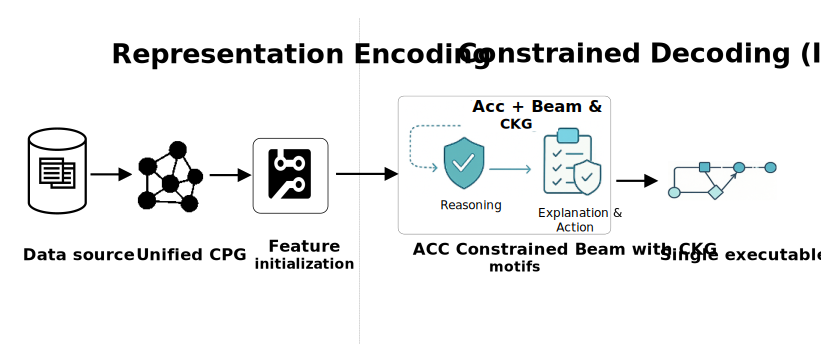
\includegraphics[width=\linewidth]{svg-inkscape/e2e.pdf}
	\caption{End-to-end pipeline for chain-centric vulnerability detection. Source repositories are parsed into a unified Code Property Graph (CPG), with GraphCodeBERT-initialized features providing input to a relation-aware encoder. At inference, ACC-constrained beam search guided by CKG motifs performs structured reasoning and outputs a single executable interprocedural chain, enabling interpretable vulnerability mechanisms.}
	\label{fig:intro-e2e-pipeline}
\end{figure}



\section{Methodological Overview and Evaluation Setup} 
\label{sec:intro-method}


This research constructs a chain-centric representation on a heterogeneous Code Property Graph that integrates Abstract Syntax Trees, Control-Flow Graphs, and Data-Flow Graphs with interprocedural semantics. The graph has call links, argument→parameter and return→caller bindings, call-site context, and conservative alias approximations. This makes it possible to move data and control between functions and files in a realistic way \cite{yamaguchi2014cpg}. Nodes and edges have features that are aware of structure. GraphCodeBERT's pretrained embeddings give hints about context and data flow \cite{guo2021graphcodebert}. A graph attention encoder collects information from different types of edges. A flow-consistency regularizer encourages attention to follow CFG-reachable def–use chains and matched call or return links while down-weighting infeasible hops.

Decoding puts together candidate chains using a limited beam search. Adaptive Causal Contextualization (ACC) makes sure that execution is possible by checking for CFG and DFG reachability, well-nested calls and returns, and alias consistency. A small Causal Knowledge Graph is only used as a score-level prior during inference and does not change the training. Supervised training improves vulnerability detection at the repository or function level and adds extra terms that encourage sparse, executable mechanisms. At inference, the system outputs a prediction along with an executable source→propagation→sink chain (\ref{sec:model-arch-gat}, \ref{sec:model-arch-ckg}, and \ref{sec:model-arch-acc} for more information).

Evaluation merges traditional classification with causal standards. Accuracy, Precision, Recall, F1, AUROC, and AUPRC are all standard metrics. The Counterfactual Consistency Score assesses the alteration of predictions in response to specific modifications of chain elements. The Causal Feature Attribution Measure tells us how much attribution mass is on sources, propagators, sanitizers, and sinks instead of off-path context \cite{Cao2024ICSE,Chu2024ISSTA,Kuang2024KSEM,Rahman2024ICSE}. These tests check for faithfulness and stability in addition to accuracy.

The experimental evaluation utilizes the ReposVul dataset~\cite{wang2024reposvul}, a repository-level benchmark meticulously crafted to reduce patch entanglement and highlight explicit interprocedural structure.  I use official project-disjoint splits without making any changes. Reproducibility is ensured by controlling preprocessing, sampling, and random seeds. I retrain baselines, such as strong graph neural detectors and a contrastive method that takes causality into account, on the same splits \cite{Zhou2019,Cao2024ICSE}. Results contain chain-centric diagnostics like length and interprocedural span, robustness checks for safe refactorings, and short case studies that show hop-level justification. This enables a direct comparison between chain-centric causal analysis and competitive learning-based baselines on both detection performance and explanation fidelity.



\section{Significance and Impact}
This research alters the explanation of vulnerabilities from localized, retrospective feature highlights to a singular, executable interprocedural causal chain that traverses from the root cause to the exploitable sink. The research makes model predictions interpretable by reconstructing how untrusted input enters the system, travels through control and data dependencies across functions, avoids or skips sanitization, and reaches a vulnerable operation. These chains give developers clear, traceable proof of a vulnerability's existence, as well as clear instructions on where to find it and what to do to fix it. This turns black-box detections into information that can be used and checked. This makes learning-based vulnerability detection more reliable, open, and useful for making sure that software is safe in the real world.

\section{Thesis Outline}
Chapter~\ref{chap:method-architecture} (Method and Architecture) formalizes the unified CPG, feature initialization, relation-aware GAT, and the ACC decoding procedure with the CKG prior; Chapter~\ref{chap:evaluation} (Evaluation Protocol and Metrics) defines conventional, chain-centric, and causal metrics and describes calibration and intervention design; Chapter~\ref{chap:results} (Experimental Results and Analysis) reports quantitative and qualitative findings, ablations (ACC/CKG/beam), decoding profile, robustness, and comparisons to \emph{COCA}; Chapter~\ref{chap:conclusion} concludes with limitations and future directions. An artifact and dataset card appear in the appendix.





%========================================
% Chapter 2 — Literature review
%========================================






\chapter{Literature Review}

The increasing reliance on machine learning (ML) to analyze source code has fundamentally transformed the software security landscape. The growing need for more reliable and interpretable vulnerability detection has driven extensive exploration of deep learning (DL) approaches. Architectures notably Graph Neural Networks (GNNs) operating over program graphs-promise scalable vulnerability detection and localization by learning structure-aware representations directly from code, often surpassing the performance of traditional static and dynamic analysis. However, despite this success, important challenges persist: difficulties generalizing across projects and distributions, high sensitivity to spurious correlations, limited support for interprocedural reasoning, and explanations that are insufficiently faithful for developer remediation. This chapter synthesizes the trajectory from early DL-based vulnerability detection and model explanation to current causality-aware approaches. I give particular attention to the development of pre-trained structural encoders and the emerging need for datasets that better reflect interprocedural mechanisms, ultimately crystallizing the unresolved gaps that motivate the core contributions of this thesis.

\section{Theoretical Foundations and Background}


Here I consolidates the key theoretical concepts and technical background necessary for understanding the research presented in this thesis. It distinguishes software bugs from security vulnerabilities, reviews classical static and dynamic analysis, details canonical code representations that enable structurally informed reasoning, explains interprocedural semantics for modeling flows across function boundaries, and motivates the incorporation of causality and counterfactual reasoning into security analytics. Where appropriate, references to recent surveys and representative systems are provided to anchor definitions and scope \cite{Chakraborty2020,Liu2020}.

\subsection{Software Bugs and Vulnerabilities}
\label{sec:intro-bugs}

A \emph{bug} is a defect that causes a program to behave incorrectly or unexpectedly. Not all bugs threaten security. A \emph{vulnerability} is a defect that an adversary can exploit to violate confidentiality, integrity, or availability. Distinguishing benign errors from exploitable vulnerabilities requires understanding not only the defect itself but also the \emph{mechanism} by which it can lead to a successful attack.

This mechanism can be conceptualized as a chain of causation that begins at a \emph{root} condition (e.g., untrusted input, unchecked buffer length, use-after-free) and \emph{propagates} through assignments, parameter passing, return values, aliasing relations, and implicit flows induced by control dependence. The chain becomes exploitable when a tainted or unsafe state reaches a sensitive \emph{sink}, such as a buffer write, command/SQL execution, deserialization routine, or privileged operation. Executability depends on dominance and post-dominance of guards, exceptional paths, resource lifetimes, and other feasibility constraints. This thesis therefore treats vulnerabilities as \emph{root$\rightarrow$propagation$\rightarrow$sink} mechanisms to be reconstructed and validated end to end.

\subsection{Classical Program Analysis: Static and Dynamic}
\label{sec:intro-classical}

\textbf{Static analysis} reasons about program behavior without execution. It uses dataflow frameworks and abstract interpretation to approximate reachable states across all paths. Precision is governed by \emph{flow sensitivity} (does the analysis respect statement order?), \emph{context sensitivity} (does it distinguish call sites or call histories?), \emph{path sensitivity} (does it track path conditions across branches?), and \emph{heap/field sensitivity} (does it distinguish fields and heap objects). Interprocedural static analysis requires constructing and resolving call graphs (e.g., class hierarchy analysis, rapid type analysis, points-to based resolution) and often employs summary-based propagation or IFDS/IDE-style solvers for scalable, distributive problems. Alias and points-to analyses are critical because they determine whether references may refer to the same memory, thereby controlling precision of def--use reasoning. Static analysis scales and can identify candidate roots, propagators, and sinks early, but coarse abstractions or under-modeled sanitization may cause false positives.

\textbf{Dynamic analysis} executes the program (or symbolic abstractions) to observe concrete behaviors. Fuzzing mutates inputs to trigger failures; sanitizers instrument code to detect memory errors and undefined behavior at runtime; concolic/symbolic execution uses path constraints to steer toward hard-to-reach states. Dynamic analysis yields concrete \emph{witness traces} but faces input-space and path-explosion limits. In practice, static analysis can prioritize likely vulnerable chains, while targeted dynamic validation confirms executability. This complementarity is especially useful for interprocedural mechanisms that cross module boundaries and depend on calling contexts.

\subsection{Code Representations for Security Analysis}
\label{sec:intro-repr}

\textbf{Abstract Syntax Tree (AST):}
The AST encodes the hierarchical syntactic structure of source code, abstracting away punctuation to represent declarations, expressions, and statements. It supports parsing, symbol resolution, and scope management. By itself, the AST lacks explicit execution ordering and data provenance, limiting its utility for end-to-end vulnerability tracing.

\textbf{Control-Flow Graph (CFG):}
A CFG represents the flow of control between basic blocks, including exceptional control. Analyses derive dominance/post-dominance, loop structure, and reachability---all necessary for judging whether guarding conditions actually protect sinks. Interprocedural CFGs (ICFGs) connect call sites to callees and returns to callers, modeling control transfer across procedures and enabling reachability checks across functions.

\textbf{Data-Flow Graph (DFG):}
A DFG links definitions to uses (def--use chains), tracking value provenance across assignments, operations, parameter passing, and returns. Static Single Assignment (SSA) form simplifies reasoning by introducing $\phi$-nodes at merges. Interprocedurally, argument$\rightarrow$parameter and return$\rightarrow$caller bindings extend provenance across calls, while alias/points-to facts determine when references share storage.

\textbf{Program Dependence Graph (PDG):}
The PDG unifies data and control dependencies in a single graph, enabling slicing along both axes and reasoning about implicit flows. PDGs are commonly intra-procedural; explicit extensions are required to model interprocedural flows for whole-program reasoning.

\textbf{Code Property Graph (CPG):}
The CPG combines AST, CFG, and DFG into a heterogeneous, typed multigraph, supporting joint queries over syntax, execution order, and data dependencies \cite{yamaguchi2014cpg}. CPGs are well suited to vulnerability discovery because they admit taint-style queries that trace feasible paths from sources through transformations to sinks while retaining syntactic anchors for precise localization. For interprocedural analysis, the CPG is enriched with call-graph edges, argument$\rightarrow$parameter and return$\rightarrow$caller links, call-site context (e.g., dynamic dispatch), and coarse alias information, enabling faithful reconstruction of cross-boundary propagation. This thesis adopts an augmented CPG as the backbone for chain-centric mechanism tracing.

\textbf{Interprocedural Semantics:}
Executable vulnerability chains often cross function boundaries. To capture these flows, the representation integrates (i) a call graph, (ii) argument-to-parameter and return-to-caller relations, (iii) call-site contexts (e.g., receiver/dispatch in object-oriented code), and (iv) alias/points-to approximations. Together they support tracing explicit data flows and implicit control effects across modules in a way that aligns with feasible program execution.


\subsection{Learning over Program Graphs}
\label{subsec:learn-over-graphs}

Learning-based techniques complement classical analysis by operating directly on structured code graphs. In this view, programs are represented as heterogeneous graphs that merge AST, CFG, and DFG into a unified Code Property Graph (CPG), exposing typed nodes/edges (e.g., \texttt{CFG}, \texttt{DFG}, \texttt{CALL}, \texttt{ARG}\(\to\)\texttt{PARAM}, \texttt{RET}\(\to\)\texttt{CALLER}). Graph neural networks (GNNs) then propagate information along these relations to classify snapshots or localize vulnerable regions, with statement/line-level variants explicitly exploiting structure to sharpen localization \cite{Zhou2019,hin2022linevd,Chakraborty2020}. Relation-aware message passing and attention over edge types are particularly well-suited to interprocedural reasoning because they can weight control-, data-, and call/return links differently during aggregation.

Structure-aware pretraining further improves node/edge representations before graph reasoning. In particular, GraphCodeBERT injects data-flow awareness into transformer encoders and yields context-sensitive token embeddings that, when fused with structural channels, improve cross-project generalization \cite{guo2021graphcodebert,fu2022linevul}. In this thesis, such frozen language-model features provide a stable semantic channel, while the relation-aware GNN learns how evidence should travel across heterogeneous edges in the CPG.

Despite these advances, empirical studies consistently show degradation under benign refactorings and cross-repository transfer, revealing sensitivity to spurious, project-specific correlations \cite{Li2022Empirical,yang2022natural}. This motivates going beyond correlation-based detectors toward mechanisms that privilege executable flows. Recent lines of work introduce causal notions at different levels: contrastive/counterfactual training and inference (\emph{COCA}, \emph{CFExplainer}) \cite{Cao2024ICSE,Chu2024ISSTA}, causal adjustment and denoising to suppress non-causal context (\emph{Snopy}) \cite{Cao2024ASE}, and structural-causal formulations that prioritize features with genuine influence (\emph{VulCausal}, \emph{CausalVul}) \cite{Kuang2024KSEM,Rahman2024ICSE}. Broader explainability studies also highlight the gap between saliency-style rationales and truly causal explanations, calling for evaluations that test faithfulness and intervention stability \cite{Allix2024,li2023xai,Moschitti2024}.

These observations motivate the chain-centric stance taken here: use a unified, interprocedural program graph; learn relation-aware evidence propagation over it; and then \emph{constrain} decoding so that the returned explanation is a single, executable root\(\rightarrow\)propagation\(\rightarrow\)sink chain. Causal priors and structured decoding (detailed next) ensure that learned scores translate into mechanisms that remain valid under program semantics and robust under counterfactual edits.







\subsection{Causal-Guided Structured Decoding}
\label{sec:theory-ckg}

\paragraph{Causal Knowledge Graph(CKG):}
\label{para:rw-constrained-ckg}

The concept of a \emph{Causal Knowledge Graph (CKG)} has emerged in recent literature as a means of capturing the underlying mechanisms that explain \emph{why} specific structural or semantic relationships tend to follow one another, rather than merely documenting their co-occurrence~\cite{Kuang2024KSEM,Cao2024ICSE}. Within program analysis, such knowledge graphs enable models to represent and reason about directional causal dependencies between program relations. Unlike traditional graph structures, which primarily record entities and factual edges, a CKG encodes empirical patterns and causal tendencies, thereby providing a foundation for more interpretable, mechanism-aware reasoning~\cite{Rahman2024ICSE,Zheng2023CausalKG}.

In the context of vulnerability detection, this thesis leverages CKGs to model causal pathways underlying interprocedural vulnerability propagation~\cite{Kuang2024KSEM,Cao2024ICSE}. Nodes in the CKG correspond to relation types within heterogeneous program graphs, such as function calls, argument-to-parameter bindings, return-to-caller edges, or data-flow and control-flow links. Directed edges represent empirically observed transitions, indicating where one relation type tends to cause or enable another during the construction of vulnerability chains. Beyond simple one-step transitions, the CKG summarizes multi-step motifs—recurrent bi-grams and tri-grams—that characterize common propagation mechanisms in actual codebases. For instance, frequent motifs may describe a function call followed by argument propagation and then a return linkage, reflecting a typical cross-functional vulnerability transfer~\cite{Rahman2024ICSE,guo2021graphcodebert}.

The value of a CKG lies in its ability to guide learning systems away from brittle, correlation-driven associations. Purely data-driven detectors risk overfitting to locally prevalent regularities that lack mechanistic grounding, resulting in poor robustness under domain shift~\cite{Li2022Empirical}. A CKG estimated post hoc from training graphs acts as a lightweight structural prior, gently nudging chain assembly toward empirically plausible transition patterns without enforcing rigid rules or handcrafted heuristics~\cite{Kuang2024KSEM,Rahman2024ICSE}. This structure regularizes the inference process, reducing uncertainty and encouraging coherent, interpretable chain construction.

Construction of a CKG relies on analyzing relational evidence from large program datasets to derive statistically frequent transition patterns between relation types. These patterns are extended into higher-order motifs, creating a compact summary of causal sequence structures across interprocedural contexts. The resulting graph reflects both likely cause-effect transitions and interpretable motifs that can be visualized or audited by developers~\cite{Kuang2024KSEM,Zheng2023CausalKG}. Importantly, the CKG operates as an auxiliary, non-intrusive source of plausibility: learned evidence from the main detection model remains paramount, with the CKG acting as a gentle regularizer that rewards transitions reflecting historically robust causal structure.

Integration of a CKG into vulnerability detection aligns with ongoing research in explainable artificial intelligence and causal inference, which prioritize mechanistic interpretability over mere statistical association~\cite{Chakraborty2020,Moschitti2024}. Prior studies highlight the pitfalls of models lacking causal grounding, noting that visual explanations derived from attention or saliency scores often misrepresent the actual factors driving a prediction~\cite{Chakraborty2020,Cao2024ASE}. By explicitly encoding directional causal patterns among program relations, the CKG supports stability and transparency in chain reconstruction. Each causal link can be contextualized within a known relational motif, making the resulting causal pathway auditable and actionable for developers~\cite{Kuang2024KSEM,Chu2024ISSTA}.

Overall, while traditional knowledge graphs serve mainly as record-keepers for observed facts, a CKG distinguishes itself by focusing on mechanistic tendencies and supporting reasoning under hypothetical interventions, such as what happens when a relation is inserted, altered, or removed. This ability to model executable vulnerability chains with explicit causal grounding positions CKGs as essential tools in mechanistic vulnerability analysis, where understanding the propagation mechanism is as important as detecting the flaw itself~\cite{Kuang2024KSEM,Cao2024ICSE,Rahman2024ICSE}.

\paragraph{Constrained Decoding and Beam Search for Structured Reasoning:}
\label{para:rw-constrained-beam}

Beam search has become a widely adopted heuristic for navigating complex structured search spaces, enabling the efficient identification of high-quality candidate solutions by maintaining a finite set of top-scoring partial hypotheses at each expansion step~\cite{RussellNorvig2020AI}. This approach balances exploration with computational tractability, making it particularly useful in combinatorial prediction tasks. In the context of structured reasoning and program analysis, however, conventional beam search and naive methods such as best-first or depth-first search often struggle with the feasibility constraints imposed by programming language semantics and logical requirements. These unconstrained strategies can produce locally optimal but globally invalid paths, resulting in interpretations or program traces that do not respect the logic of the system.

The concept of \emph{constrained decoding}, also known as guided beam search, addresses this limitation by enforcing domain-specific validity criteria during the search process~\cite{Martins2022StructuredDecoding}. In constrained beam search, candidate expansions are dynamically filtered or weighted based on both hard structural constraints (e.g., grammar rules, type safety, execution order) and soft statistical preferences drawn from prior knowledge or data. For program graph reasoning, these constraints typically include control- and data-flow consistency, legality of interprocedural transitions (such as proper function call/return matching), avoidance of cycles or infinite recursion, and aliasing concerns. Incorporating these checks ensures the resulting reasoning chains or traces correspond to paths that are executable and semantically valid, preserving logical coherence across function and module boundaries~\cite{Chu2024ISSTA}.

Practical applications of constrained beam search span diverse structured prediction problems such as syntactic parsing~\cite{Freitag2017Parsing}, symbolic program execution~\cite{Li2022Empirical}, knowledge graph inference, and code generation. Earlier methods often relied on hand-crafted heuristics or deterministic rules for pruning search paths, while others introduced scoring functions based on local learned features. However, exclusive dependence on heuristics can fail to adapt across domains, and purely data-driven scoring may lack generalizability and fall prey to spurious correlations. Addressing these shortcomings, recent research integrates statistical priors mined from empirical data, such as edge-gram or motif frequencies directly into the decoding process. These data-driven priors help guide the search toward patterns historically associated with correctness, blending empirical knowledge with strict legality filters~\cite{Kuang2024KSEM,Rahman2024ICSE}.

Compared to more global but computationally intensive optimization methods like Integer Linear Programming (ILP) or Satisfiability Modulo Theory (SMT) solving, constrained beam search achieves a practical and interpretable compromise~\cite{mandal2020solving}. It enables efficient exploration of numerous plausible causal chains, generating a ranked collection of candidate explanations suitable for developer inspection and verification. The synergy between legal constraint enforcement and empirical causal priors produces a decoding process that is both mechanism-aware and computationally tractable, thereby supporting the broader goal of generating structured, executable explanations that faithfully represent how vulnerabilities propagate in complex software systems.




\section{Related Works}

\subsection{Static Analysis: Foundations and DL Integration}

Static analysis examines software artifacts without executing them, reasoning exhaustively about possible program behaviors through frameworks like lattice-based dataflow analysis and abstract interpretation \cite{yamaguchi2014cpg, Chakraborty2020}. Its precision depends on sensitivities to control flow, call context, execution paths, and heap or field representations. Interprocedural static analysis demands accurate call graph construction, supported by methods such as Class Hierarchy Analysis, Rapid Type Analysis, and points-to analyses to resolve aliasing \cite{Xia2023, Liu2020}.

These analyses utilize canonical program representations: Abstract Syntax Trees (ASTs) encode syntactic structure; Control-Flow Graphs (CFGs) model executable order and branching; Data-Flow Graphs (DFGs) trace variable value definitions and uses; and Program Dependence Graphs (PDGs) unify data and control dependencies for program slicing. The Code Property Graph (CPG) integrates AST, CFG, and DFG into a heterogeneous multigraph that supports global queries essential for interprocedural taint tracking from sources to sinks \cite{yamaguchi2014cpg}.

Despite early identification benefits, classical static analysis suffers from false positives due to over-approximation in modeling sanitizers, aliasing, and dynamic dispatch \cite{Ruiz2023, Marchetto2024}. Automated static analyzers such as Flawfinder, RATS, CPPCheck, SpotBugs, and PMD show variability in detection accuracy and false positive rates across languages like C++ and Java \cite{Kaur2020comparative}. These limitations motivate the development of DL-augmented static analysis tools. For example, IRIS incorporates large language models (LLMs) with static analysis to infer taint specifications and improve vulnerability detection coverage and false discovery rates, surpassing traditional tools like CodeQL \cite{Li2024IRIS}.

Further, hybrid approaches blend static analysis with ML classifiers to filter and prioritize warnings, addressing false positives and improving scalability \cite{hu2023hybrid}. Static analysis remains foundational, providing structured input to DL models, yet its limitations in handling complex, evolving, and domain-specific codebases remain a persistent challenge \cite{Xia2023, Chakraborty2020}.

\subsection{Dynamic Analysis: Execution Evidence and DL Integration}
Dynamic analysis observes real or symbolic execution of programs with concrete inputs to detect vulnerabilities manifesting during runtime \cite{yagemann2021arcus, yagemann2021automated}. Techniques include fuzzing, which automates input mutation to explore program paths; sanitizers, which instrument binaries or source to catch memory errors; and symbolic or concolic execution, which employs solvers to systematically explore feasible paths leading to fault states.

Dynamic methods provide high precision witness traces, essential for actionable debugging, but suffer from path explosion and limited environmental coverage, particularly in large interprocedural contexts \cite{yagemann2021arcus}. This gap has incentivized hybrid strategies integrating machine learning to guide input generation or prioritize suspicious execution traces, enhancing coverage efficiency \cite{xu2023mlforfuzzing}.

Recent work employs reinforcement learning and deep models to optimize fuzzing or dynamic analysis workflows, combining symbolic constraints and learned heuristics to uncover hard-to-detect vulnerabilities \cite{tufano2022adaptive}. These advances promise better balancing precision and exploration in complex, modern software systems.

Dynamic analysis's concreteness complements static analysis’s scalability, and their integration with machine learning techniques is an active research frontier poised to improve vulnerability detection coverage, efficiency, and interpretability.



\subsection{Deep Learning Based Techniques}

Deep learning is transforming many areas of computer science and has been applied in research projects. In particular, graph neural networks (GNNs) \cite{hin2022linevd}, deep learning models have rapidly shown their promise in vulnerability detection, achieving amazing precision in identifying susceptible code patterns \cite{chakraborty2021deep, Liu2020, Yaqin2020}. GNNs offer a natural approach for capturing complex software dependencies by modeling code as graphs, using nodes for elements (e.g., variables, functions) and edges for relationships (e.g., data flow, control flow). Hin et al. \cite{hin2022linevd}, for instance, showed how well GNNs identified vulnerabilities at the statement level. With the capacity to learn from the structure and semantic information of code, the models were able to spot vulnerabilities suggestive of buffer overflows or injection issues. Although many of these early deep learning models functioned as "black boxes," impairing the knowledge of their decision-making processes \cite{li2023vulanalyzer, mosolygo2021towards}, even with their precision. Especially in the context of software security, the ability to understand the reason \emph{why} a model finds a piece of code as vulnerable is crucial for developers to implement fixes \cite{USGov2023}. This lack of transparency is a major concern. Furthermore, impeding the acceptance of these approaches in practical software development processes is their difficulty in explaining model predictions. The US Government's executive order \cite{USGov2023} on the safe, secure, and trustworthy development and use of artificial intelligence emphasizes how much artificial intelligence (AI) is becoming relied upon in important systems, where erroneous or untrustworthy predictions can have severe consequences.

Zhou et al. \cite{Zhou2019} presented a comprehensive comparative analysis of factors influencing the performance of deep learning (DL)-based vulnerability detection systems. Recognizing the complexity of software vulnerabilities, the authors sought to systematically evaluate how different design choices affect detection efficacy. To this end, they constructed two distinct datasets, capturing both data reliance and control dependencies extracted from programs, encompassing a diverse set of 126 different vulnerability types. Their methodology involved assessing the quantitative impact of several key elements on vulnerability identification performance. This included employing techniques for handling unbalanced data, incorporating control dependence information within code representations, and experimenting with various neural network architectures. To facilitate their analysis, Zhou et al. built a DL-based vulnerability detection system leveraging Joern, an expanded open-source code parser. The primary contribution of this work lies in its systematic assessment of the quantitative influence of these elements on vulnerability detection efficacy. The study's results offer valuable insights into the design and development of effective deep learning-based vulnerability detection systems. However, it's important to note that this research did not specifically address causal deep learning (CDL) or explicitly incorporate causal reasoning principles. The authors themselves highlighted the need to accommodate a wider range of vulnerability types, enhance the representation of code features, and overcome the limitations of relying solely on control and data dependencies. 

Li et al. \cite{Li2022Empirical} performed empirical research on deep learning (DL) models for vulnerability detection. On Devign and MSR data, they polled and replicated nine state-of-the-art (SOTA) models. They looked at and examined model capabilities (agreement, variability, performance on several vulnerability categories, and difficulties in addressing particular code aspects). They investigated how model performance responded to project mix and training data size. They identified significant code aspects applied for prediction using model explanation tools. The main contribution of the writers was a thorough investigation of models of deep learning vulnerability detection. For assessing and contrasting several deep learning models for vulnerability identification, this research offers a useful standard. Still, this study paid little attention to causative factors. The writers urged more investigation on code patterns, possible inclusion of causal detection for better generalization, and addressing of the shortcomings of present model interpretation techniques.

Zou et al. \cite{Zou2020} tackled this problem with domain adaptation methods and deep learning. To reduce distribution discrepancies between domains, their CD-VulD system learnt cross-domain representations. Learning token embeddings for generalization across tokens, the CD-VulD system transforms software program representations into token sequences. Abstract high-level representations based on those sequences are built using a deep feature model. Minimizing the distribution divergence between the source and destination domains helps to train cross-domain representations using the metric transfer learning framework (MTLF). The key contribution of the authors was a CD-VulD system learning cross-domain representations of source code via domain adaptation and deep learning. Practical vulnerability identification depends on generalizing across several fields, as models trained on one dataset might not work on another. This research did not, however, use causal reasoning; the authors observed constraints in evaluation scope and dependency on particular architectures.

\subsection{Causal Reasoning and Causal Deep Learning Techniques}

Conventional deep learning techniques have shortcomings, including their capacity to detect erroneous correlations and changes in dataset distribution. Stronger and broader methods have emerged from this. VulCausal, developed by Kuang et al. \cite{Kuang2024KSEM}, solves what caused what in neural network models. Finding and eliminating bogus links between API functions, user-defined names, and code structure is VulCausal's primary objective. The authors provide a structural cause model to demonstrate how discovering vulnerabilities is affected by user-defined names, API library IDs, and code structure. The study employs covert adjustment in the reasoning stage to eliminate erroneous correlations and minimize the impact of confounders. By modeling and lowering spurious correlations, VulCausal aims to make vulnerability identification more accurate and consistent than conventional deep learning approaches. This is a crucial first step toward exposing vulnerabilities. The writers mostly included a causal perspective to eliminate misleading correlations and provide more accurate and reliable vulnerability detection. When causal inference techniques were developed, they connected with a whole new level and helped us to better understand the factors causing vulnerability in individuals. One significant fresh concept is the application of backdoor correction and causal reasoning approaches. The approach wasn't flawless, the writers noted, though, as it lacked scalability to extremely big codebases, it wasn't ubiquitous across many computer languages, and it couldn't show direct causality (beyond performance benefits). This indicates that in these fields additional research is required. One should also consider the extent of labour causal inference techniques demand and the requirement of well crafted models. Zelikman et al. \cite{Zelikman2023} on self-taught optimizers also indicate that individuals are still striving to create machine learning models that are more efficient and helpful.

Le et al. \cite{Le2024MBU} investigated how well existing deep learning-based detectors could handle vulnerabilities spanning several base units of code (MBUs). Their empirical evaluation of current deep learning-based detectors revealed a clear deficiency in tackling MBU vulnerabilities, usually overstretching accuracy by focusing on individual base units (IBUs). Although it did not specifically include causal reasoning in the detection technique, this research underlined the need of investigating the features and distribution of MBU vulnerabilities as well as the limits of current datasets. Together with a detailed analysis of their incidence and detection accuracy in modern deep learning (DL)-based detectors, the authors gave a description and categorization of MBU vulnerabilities. The key contribution of the authors was the proposal of a framework for the correct integration of MBU vulnerabilities in DL-based detection. The study emphasizes the significance of evaluating the spectrum of vulnerabilities and of studying detection methods. The problem of MBU vulnerabilities is particularly relevant in modern software development, as code usually involves numerous files and modules. Furthermore, improving the understanding of vulnerability types and their frequency is the research by Nong et al. \cite{Nong2023ICSE} on authentic vulnerability generation through pattern mining and deep learning and the study by Woo et al. \cite{Woo2023USENIX} on identifying 1-day vulnerabilities in reused open-source software components.

Cao et al. \cite{Cao2024ASE} proposed Snopy, a deep learning (DL)-based technique bridging sample denoising with causal graph learning to enhance vulnerability identification. Snopy expressly included causal reasoning utilizing a Causality-Aware Graph Attention Network (CA-GAT), a Feature Caching Scheme (FCS), and a Causality-Aware Graph Attention Network (CA-GAT) identifying bogus features. Though areas for future research remain, including generalizability to other programming languages and vulnerability types \cite{Woo2023USENIX} and more sophisticated ways for mitigating spurious correlations in code, this approach represented a major step toward causal vulnerability detection. Initially, deleting vulnerability-irrelevant code elements and constructs using change-based sample denoising and then developing a Causality-Aware Graph Attention Network (CA-GAT) utilizing Feature Caching Scheme (FCS), Snopy learns causal vulnerability traits. The main contribution of the authors was a change-based method guided by vulnerability-fixing commits (VFCs) automatically removing vulnerability-irrelevant code components. A unique addition is made by the combination of sample denoising with causal graph learning; the usage of VFCs offers a moral approach to finding and eliminating pointless code components. Building strong and dependable vulnerability detection systems depends on one being able to differentiate between causal and spurious aspects.

Ganz et al. \cite{Ganz2024} focused on addressing data quality, model interpretability, robustness, and contextual sensitivity, thereby enhancing the usefulness of machine learning (ML)-driven vulnerability identification. This research particularly applied causal learning approaches to reduce confusing effects and improve detection robustness. They developed datasets by using a novel neural code augmentation technique. They assessed explanation tactics using a novel approach based on dynamic program analysis. They assessed models on their acquired biases using a novel assessment system based on causal learning. The main contribution of the authors was to provide strategies raising the relevance of learning-based vulnerability detection in practical environments. The study underlines the need to attend to pragmatic issues such as data quality and model interpretability. Relevant to the problems of model interpretability and explainability is the research by Suneja et al. \cite{suneja2021probing} on evaluating model signal-awareness by means of prediction-preserving input minimization, together with the study by Yu et al. \cite{yu2023counterfactual}.

Growing interest in causal deep learning (CDL) results from the limits of current approaches, especially in terms of generalization and the capacity to find the underlying causes of vulnerabilities. By means of CausalVul, Rahman et al. \cite{Rahman2024ICSE} directly addressed the lack of resilience and generalization to out-of-distribution (OD) data in deep learning (DL)-based vulnerability detection. Explicitly leveraging do-calculus and the backdoor criterion, this two-stage approach aimed at identifying and eliminating false features using causal learning algorithms. This paper clearly shows a clear improvement in causal deep learning (CDL) for vulnerability detection, therefore highlighting the possibilities of causal inference to increase model generalization. The correlations between code features and the vulnerability label were shown by the authors using a causal graph. They then trained models that were less dependent on spurious features and more focused on causal features by the use of do-calculus and the backdoor criterion. The main contribution of the authors was to explicitly address false correlations, thereby introducing a fresh method to increase the generalization and resilience of deep learning (DL)-based vulnerability detection. Two important developments are the application of the backdoor criterion and do-calculus. Real-world applications depend on generalizing OOD data since the spread of vulnerabilities may evolve with time.

Chu et al. \cite{Chu2024ISSTA} addressed the lack of explainability in Graph Neural Networks (GNNs) for vulnerability identification. Using counterfactual reasoning, a type of causal inference, CFExplainer aimed to identify minimal changes to the input code graph that would influence the GNN prediction. This improved explainability by focusing on behaviours that alter the outcome and so provides a "what-if" analytical capability. The approach finds a minimum disruption in the code graph by inverting the prediction of the GNN. This provides developers with useful knowledge and guides them on the necessary changes to eliminate a vulnerability. The authors mostly contributed by developing a counterfactual explanation method for GNN-based vulnerability discovery. Counterfactual thinking helps developers find a more reasonable and workable argument. A better basis for understanding the application of counterfactual reasoning in explainable artificial intelligence is provided by the work of Lucic et al. \cite{lucic2022cf}.

Islam et al. \cite{Islam2024} presented T5-GCN for vulnerability categorization, localization, and root cause identification. Although the "root cause" was sought for, this research did not specifically use causal deep learning (CDL), causal inference, or causal reasoning methods. Conversely, the explainability part of T5-GCN aims to identify the "root cause" of vulnerabilities, therefore indirectly guiding knowledge of the elements generating the vulnerability. The approach uses DeepLift-SHAP attribution values to determine the relevance of tokens in the code, therefore identifying the basic cause. Along with their classification, location, and a brief static description, the writers mostly contributed a method employing explainable methodologies to identify the root cause of a vulnerability. One original method is to combine GCNs and LLMs. Large language models (LLMs) for code analysis are a fast-expanding field of research; the research of Zelikman et al. Furthermore underlined in \cite{Zelikman2023} on self-taught optimizers, the potential of LLMs in this field is relevant for the application of LLMs in code analysis, and vulnerability detection is the effort of Pearce et al. \cite{pearce2025asleep} to assess the code contributions' security of GitHub Copilot.

Cao et al. \cite{Cao2024ICSE} presented Coca, a framework to enhance the causality and robustness of Graph Neural Networks (GNNs)-based vulnerability detection systems. Coca used dual-view causal inference, that is, factual and counterfactual reasoning, to pinpoint code statements most likely to be decisive for vulnerability discovery. This method showed a sophisticated use of causal ideas to solve constraints in robustness and explainability observed in past GNN-based detectors. It also underlined the difficulties in juggling concision with effectiveness in explanations. Coca trains GNNs less prone to false correlations and more focused on real vulnerability traits by means of combinatorial contrastive learning. The Explainer component generates succinct and powerful explanations using dual-view causal inference. Using supervised constrastive learning, the system is taught to identify the bug in all versions and distinguish between buggy and non-buggy code. It discovers a flaw and then employs factual and counterfactual thinking. This is a framework enhancing the causality and dependability of GNN-based vulnerability detection systems. 

\subsection{Explainability and Interpretability Techniques}

In the first attempt to tackle the explainability issue, scientists aimed to create techniques that would reveal the inner workings of deep learning models, hence enabling more reasonable and reliable predictions. Proposed by Le et al. \cite{li2023vulanalyzer}, GAVulExplainer was one of the first attempts to handle this using a model-agnostic approach, that is, one can apply GAVulExplainer to several deep learning models and genetic algorithms to help find important subgraphs causing vulnerabilities. The basic concept is to build a subgraph emphasizing the important elements causing the vulnerability, therefore offering a more understandable justification for the predictions of the model. While avoiding local optima, the genetic algorithms effectively seek accurate substructure information. This method employs a fidelity metric to assess the quality of produced explanations and lets users regulate the size of the explanation subgraph. GAVulExplainer marks a significant progress in enhancing the interpretability of GNN-based vulnerability detection, but it still lacks explicit modeling of the fundamental \emph{causal} links between code characteristics and vulnerabilities. Finding contributing subgraphs still takes front stage without exploring causal deep learning (CDL) methods. Furthermore, its assessment depends on fidelity criteria, which might not completely reflect the pragmatic value of the explanations for developers in real-world debugging situations, especially given the complexity of software systems and the several ways vulnerabilities might show themselves. This study addressed the demand for explainable prediction since they realized that successful remedial action and developer confidence depend on knowing the "why" behind the prediction of a model.

Li et al. \cite{li2023vulanalyzer} presented that Vulanalyzer is another significant initiative aimed at improving explainability. Specifically developed for binary detection, a rather difficult subject given the low-level features of binary code, this deep learning model, Vulanalyzer, accurately preserves instruction semantics and structural linkages by using sequential and topological learning to mimic program execution through recurrent units and graph convolution, especially in assembly code \cite{taviss2024asm2seq}. Mostly distinguished by its multi-head attention system, which stresses pertinent commands and fundamental blocks, Vulanalyzer underlines fundamental directions and basic blocks. This encourages developers to concentrate on the code components the model considers most indicative of a vulnerability, therefore producing interpretable results. Although it clarifies things, Vulanalyzer, like GAVulExplainer, does not especially mix causal reasoning, causal inference, or causal deep learning (CDL). Emphasizing the need of greater study on causal approaches that can identify the why behind vulnerability projections, the emphasis stayed on simplifying difficult interactions and improving interpretability by means of attention processes. The writers mostly concentrated on the lack of explainability and the challenges to elucidate intricate links in binary code. With topological and sequential learning combined, the approach captures structural relationships as well as instructional meanings, so requiring minimal topic knowledge. Still, even if attention processes help to define the what of the model's judgments, they do not naturally define the \emph{why} - the fundamental causal factors generating the sensitivity. Most importantly, the method can be applied over multiple architectures and code obfuscation methods. The research on the development of explainable functional summaries of assembly code performed by Taviss et al. \cite{taviss2024asm2seq} emphasizes understanding code semantics in vulnerability analysis.

Moschitti et al. \cite{Moschitti2024} presented an XAI-based system for assessing computer code in a graph environment. This system evaluates the significance of syntactic structures for Common Weakness Enumeration (CWE) classification \cite{li2023xai}, therefore connecting learnt code feature representations to subtle semantics recognized by security professionals. The system generates ranks of syntactic constructive contribution levels in Abstract Syntactic Trees (AST) among CWE types for Java and C++ datasets. A novel feature-masking method, varying the neighbourhood of code tokens and syntactic constructions, is applied for the graph environment. The change in the code token neighbourhood is transformed into the CWE-type similarity score by means of information retrieval approaches. The authors showed how nuanced semantics understood by security professionals might be connected to the learnt code feature representations by CWE similarity generated from XAI explanations. This approach did not, however, particularly target causal reasoning or causal deep learning (CDL). The authors admitted that present XAI systems have several limits, namely, their incapacity to generalize to undiscovered vulnerability patterns and transcend the scope of input data. The constraints covered are those of interpretability of acquired features and transferability of learned patterns to different datasets. Although graph-based representations and ASTs are widely used in vulnerability identification, their efficacy may vary depending on the programming language and the particular vulnerabilities under attack. The research of Allamanis et al. \cite{Xia2023} on machine learning for massive code and naturalness offers a larger background for appreciating the difficulties of expressing and evaluating code.

Hajipour et al. \cite{Hajipour2023} developed a framework for vulnerability threat prediction. This method generated a semantic representation and computed an explainable threat score by prioritizing research activities using topic modeling of vulnerability descriptions (from sources like the National Vulnerability Database). Furthermore, included was a fresh trend score based on internet infosec conversations to pinpoint popular vulnerabilities. These results were aggregated on a visual dashboard to give investigative work top priority. The main contribution of the authors was the computation of a new trend score and an explainable threat score based on the topic model. This framework offers a semantic representation of vulnerabilities constructed using topic modeling of vulnerability descriptions. The framework offers a semantic representation of vulnerabilities constructed using topic modeling of vulnerability descriptions. Although helpful for prioritizing, it did not investigate the fundamental \emph{causal} elements affecting vulnerability exploitability, like particular code patterns or interactions increasing the probability of the exploitation of a vulnerability. Understanding which vulnerabilities are most likely to be exploited aids in prioritizing risk management efforts. Existing frameworks often rely on online discussions and external vulnerability descriptions, which may introduce biases and limit timeliness and completeness.

Allix et al. \cite{Allix2024} investigated the use of deep learning and explainability methods (most especially SHAP) toward this aim. Their results showed that explainability techniques might occasionally present distracting information, therefore harming rather than supporting engineers; code characteristics employed by DL models were often only partially connected to the underlying causes of vulnerabilities. This emphasized the need for more accurate localization and the incorporation of causal reasoning to uncover the true underlying causes. This allows for a deeper understanding that goes beyond mere correlations. The main contribution of the authors was to assess how well explainability and deep learning (DL) approaches could localize source code assertions concerning vulnerabilities. Using two deep learning (DL) techniques, VulDeePecker and JavaBert, the authors localized source code phrases pertaining to vulnerabilities using SHAP, a model-agnostic explainability method. The paper emphasizes that current explainability methods do not provide developers with practical insights effectively. Important determinants of the results of the study are the choice of deep learning models (VulDeePecker and JavaBert) and the respective application of SHAP. Practical implementations depend critically on more programming language-oriented encoding approaches recommended by Allix et al. \cite{Allix2024} and the evolution of more advanced techniques for vulnerability localization.


\section{Research Gaps}

Deep learning has made it easier to find vulnerabilities, but it still isn't very reliable, generalizable, or actionable. These deficiencies drive this endeavour.

\medskip

\noindent\textbf{Causal deficiency and generalization:}
A lot of detectors learn correlations instead of causes. They frequently fail during harmless refactorings and between projects. Normalization and domain adaptation are only somewhat helpful. Predictions continue to be erratic and do not accurately represent the fundamental flaw mechanism.

\noindent\textbf{Interprocedural reasoning:}
Most methods look at just one function or a small part of a function. They don't link root cause to propagation and sink.  Without clear cross-function control and data links, outputs stay local and don't have a clear story for how to fix them.

\noindent\textbf{Evaluation:}
Accuracy, Precision, Recall, and F1 are some of the most common metrics that only measure label agreement.  They don't check for causal faithfulness or stability when changes are made on purpose. A shared set of causal metrics is still missing.

A better method needs to learn and test how things cause each other. It ought to rebuild source-to-sink chains across functions, employ graph-based representations of program structure and evaluate behaviour through counterfactual tests and chain-aware attribution.


\section{Research Challenges and Rationale}
\label{sec:litreview-challenges}

Automated vulnerability detection has progressed, but reliability and interpretability continue to be constrained. Public corpora have almost identical entries, weak labels, and a big difference in class sizes, which makes reported accuracy seem higher than it really is and makes it harder to replicate \cite{Li2022Empirical,Chakraborty2020}. A lot of datasets only show function snippets and don't show cross-function flows. ReposVul enhances curation by maintaining repository context and call relationships \cite{wang2024reposvul}.

Representation is key. Sequence models do well on benchmarks, but they don't take into account control and data dependencies that make them easy to exploit \cite{Chakraborty2020,fu2022linevul}. Graph views (AST, CFG, DFG, PDG, CPG) represent structure \cite{Zhou2019}, but outcomes are contingent on interprocedural specifics: calls, argument-to-parameter associations, return bindings, and alias estimations. GraphCodeBERT is an example of structure-aware pretraining that adds data-flow signals to token embeddings \cite{guo2021graphcodebert}. However, the benefits depend on the level of detail and coverage.


It's hard to make executable chains from root to sink.  Unconstrained search drifts, and global solvers cost a lot.  This project employs constrained beam search in conjunction with Adaptive Causal Contextualization (ACC). The decoder will only let steps that pass reachability, call/return discipline, and alias checks through. A small causal prior (CKG), derived from relation $n$-grams, influences choices without compromising validity.

Models are fragile across projects, time, and refactorings \cite{Li2022Empirical}. Small changes that don't change the meaning can change predictions. Post-hoc explanations frequently emphasize misleading cues \cite{Allix2024,Moschitti2024}. Recent causal directions, such as counterfactual training and graph edits, enhance robustness but lack agreed-upon metrics for causal fidelity \cite{Cao2024ICSE,Chu2024ISSTA,Rahman2024ICSE,Kuang2024KSEM,Cao2024ASE}.

This thesis addresses these deficiencies. Programs are written as enhanced CPGs with clear semantics that cross boundaries. Decoding puts together a single, executable chain from the source to the sink. Evaluation uses standard detection metrics and causal tests, such as counterfactual consistency, directional agreement, on-chain attribution, and chain invalidation.



\chapter{Methodology}
\label{chap:method-architecture}

This chapter shows the learning pipeline that was used in this thesis. The objectives are twofold: precise identification of vulnerabilities and accurate reconstruction of executable interprocedural chains. The method connects a root cause to its spread and its end point through paths that don't interfere with the program's execution. This talks about the problems with models that draw lines in isolation and don't take into account how they work.

I work with an enhanced program graph. I use a Code Property Graph to show programs. This is a joint, labelled graph that combines the Abstract Syntax Tree (AST), Control Flow Graph (CFG), and Data Flow Graph (DFG) into one searchable structure \cite{yamaguchi2014cpg}. I add interprocedural links to the base CPG, such as CALL, ARG→PARAM, and RET→CALLER/RET→LHS, as well as alias summaries. This addition keeps the execution semantics the same across function boundaries and makes it possible to slice precisely for chain reconstruction.

There are three steps in the pipeline. To start, feature initialization uses GraphCodeBERT to encode tokens with context that knows about structure and data flow \cite{guo2021graphcodebert}. Pretraining on a large scale gives you useful information that you can use for later learning.  Secondly, a graph attention encoder collects signals from different parts of the graph that are close to each other. Executable relations like def–use and control dependencies guide attention. Regularization that focuses on causality lowers the need for false correlations and makes generalization better \cite{Cao2024ICSE,Rahman2024ICSE,Kuang2024KSEM}. Third, Adaptive Causal Contextualization (ACC) puts together an executable chain by choosing paths that are limited.  It makes sure that data and control are possible, follows the call-return structure, and prefers short explanations. The end result is a single chain that can be understood and matches real execution.

Training includes a classification loss for detection and penalties that make it less likely that attention patterns will be non-executable or incoherent. The learned representations maintain stability during benign refactorings and facilitate transfer across projects and programming languages. The design is based on new developments in structure-aware vulnerability detection and learning to represent causes \cite{Zhou2019,Li2022Empirical,Cao2024ASE,Chu2024ISSTA,hin2022linevd}.

The rest of the chapter talks about the formal setting, the optimization, and the algorithms for each step.  

\section{Chain-Centric Program Representation}
\label{sec:chain-conts}
\subsection{Dataset Description, Ground Truth Formation, and Preprocessing Pipeline}
\label{subsec:data-gt}

This section specifies the experimental corpus, the ground-truth labelling protocol, and the preprocessing that transforms repositories into chain-centric interprocedural graphs. I utilize \emph{ReposVul}, a repository-level dataset that separates patches, maintains multi-granularity dependencies, and eliminates outdated fixes \cite{wang2024reposvul}.


\subsection{ReposVul: scope and characteristics}
\label{subsec:reposvul-scope}

\emph{ReposVul} links CVE/CWE records to pre- and post-fix code snapshots, patch commits, and repository context \cite{wang2024reposvul}. Each entry pairs an identified weakness and severity with the exact commit, message, files, and diffs that implement the fix. Corpus construction crawls public sources, untangles mixed commits to keep only fix-relevant files, mines cross-file caller–callee relations, and filters superseded patches by commit history. The result is a repository-level view that preserves chronology, captures interprocedural links, and supports chain-centric evaluation.

\begin{table}[H]
	\centering
	\small
	\caption{Core metadata recorded per ReposVul entry.}
	\label{tab:reposvul-fields}
	\begin{tabular}{p{0.3\linewidth} p{0.65\linewidth}}
		\toprule
		\textbf{Category} & \textbf{Representative fields} \\
		\midrule
		Vulnerability entry & CVE-ID, CWE-ID, language, external references, CVE description, publish date, CVSS vector (AV, AC, PR, UI, S, C, I, A) \\
		Patch metadata & Commit ID, commit message and date, project/repository IDs, parent/child links, forge URLs \\
		Related files & File name, language, vulnerable/fixed snapshots, line diffs, file URLs \\
		\bottomrule
	\end{tabular}
\end{table}




\subsection{Extraction and graph construction pipeline}
\label{subsec:graph-construction}

The conversion from raw dataset entries to chain-centric program graphs occurs over six sequential stages.

\setlength{\fboxsep}{0pt}     
\setlength{\fboxrule}{0.3pt}  
\begin{figure}[H]
	\centering
	\includegraphics[width=\linewidth]{svg-inkscape/datasetpipeline.pdf}
	\caption{ReposVul prepossessing to interprocedural CPGs and leakage-safe train/valid/test partitions.}
	\label{fig:method-datapipeline}
\end{figure}

\paragraph{Stage A: Getting raw vulnerability and patch information:}
I add CVE/CWE metadata to \emph{ReposVul} entries and get the repository at parent and child commits. This keeps all of the pre- and post-fix files. For traceability, commit IDs, messages, dates, project IDs, and file paths are all indexed.

\paragraph{Stage B: figuring out the vulnerabilities:}
Patches often combine fixes with changes to the code. I use the corpus untangling rule, which combines model judgments with static cues, to keep only files that are relevant to fixing. 

\paragraph{Stage C: extraction of dependencies at multiple levels of granularity:}
For retained patches, I get links between callers and callees from all over the repository. When necessary, the scope includes top-level functions so that interprocedural paths from candidate sources to sinks can be recorded.

\paragraph{Stage D: making the code more consistent and building the static graph:}
For each snapshot, I make a heterogeneous program graph that combines AST, CFG, DFG, call edges, ARG→PARAM, and RET→CALLER links. Pointer and container def-use are similar to conservative alias relations. Identifiers are made anonymous, and literals are put into buckets to cut down on the differences between harmless edits \cite{Chakraborty2020,Li2022Empirical}.

\paragraph{Stage E: differencing that takes patches into account and slice materialization:}
I calculate line diffs for each patch and then create four synchronized views: changed lines, enclosing functions, touched files, and a repository subgraph that can reach any sink through possible control and data flow. These views are what you use to put together a chain.

\paragraph{Stage F: filtering based on traces for old patches:}
I keep track of file paths and commit times so I can get rid of files that don't work and patches that are no longer needed.

\begin{table}[H]
\centering
\caption{Preparation pipeline summary.}
\label{tab:pipeline}
\begin{tabular}{p{0.20\linewidth} p{0.75\linewidth}}
\toprule
\textbf{Stage} & \textbf{Key operations and outputs} \\
\midrule
A & Ingest CVE, CWE, and patch metadata; fetch pre- and post-fix files; index commits and file paths. \\
B & Apply joint untangling to retain vulnerability-fixing files. \\
C & Extract repository-level caller–callee links; expand to top-level functions when needed. \\
D & Build AST, CFG, and DFG with call and return links; attach argument$\rightarrow$parameter, return$\rightarrow$caller, and alias edges; type nodes and edges; normalize code. \\
E & Compute line deltas; assemble synchronized line, function, file, and repository subgraphs that preserve feasible paths to sinks. \\
F & Remove outdated patches using path and commit chronology; keep only current fixes. \\
\bottomrule
\end{tabular}
\end{table}


\subsection{Unified multigraph, typing, features, and storage}
\label{subsec:unified-mg}

I depict each repository snapshot as a heterogeneous multigraph constructed upon the Code Property Graph (CPG) abstraction \cite{yamaguchi2014cpg}. A single typed node store keeps program parts. Relation-specific edge sets encode \textsc{AST}, \textsc{CFG}, and \textsc{DFG}. Interprocedural links are CALL (caller to callee entry), ARG2PARAM (actual to formal), RET2CALL (callee return to call site), and RET2LHS (return value to assignment target). For all families, reverse edges are made real. This topology shows the control and data dependencies and cross-boundary flows that are needed to rebuild the chain.

For example, an identifier, literal, operator, statement, basic block, or function can be used to type nodes. Each node has a small structural feature vector that includes flags for token categories, simplified SSA indices, type hints, and normalization markers. Edges are classified by family and orientation. Optional fields include guard predicates on CFG edges and alias provenance on links that come from points-to. Shard files hold graphs, and each graph has its own metadata, such as the repository, commit, file path, and function names. This makes it possible to store things in a way that can grow and look up their origins quickly.

I keep two encodings going at the same time. The \emph{base} encoding has only small structural features for ablations and classical GNNs. The "pretrained" encoding adds a 768-dimensional embedding from GraphCodeBERT \cite{guo2021graphcodebert} to each node. The outcome is a dual-channel configuration: a low-dimensional structural vector combined with a high-dimensional contextual vector. The topology and interprocedural counts are the same for all encodings; only the feature space is different.

The set of relation types is treated as a fixed alphabet $\mathcal{R}$ by decoding. This includes \textsc{AST}, \textsc{CFG}, \textsc{DFG}, \textsc{CALL}, \textsc{ARG2PARAM}, \textsc{RET2CALL}, \textsc{RET2LHS}, and \textsc{DFG\_THIN}. It changes the weights of acceptable expansions during decoding, but it never changes the graph.



\subsection{Ground-truth definition}
\label{subsec:gt-definition}

I define ground truth on two levels. A repository revision is vulnerable at the label level if it is part of a vulnerability–fix pair in \emph{ReposVul}; the corresponding fixed revision is not vulnerable \cite{wang2024reposvul}. Using paired revisions with the same context makes it less likely that unrelated edits will confuse things.

At the mechanism level, each positive example has one executable chain that goes from a source to a sink, passing through any propagators and optional sanitizers along the way. Chains can go across function boundaries. Sources are places where data that can't be trusted gets into the program state, like when it parses input or deserializes it. Sanitizers check or limit that state, like checks for bounds or checks for correct format. Propagators move taint through assignments, passing parameters, returns, pointer hops, container writes, or index arithmetic. When you reach a sink, it becomes an exploitable operation that is important for security. Examples include memory writes, command execution, path traversal, database calls, and unsafe casts. Lexicon and patterns can be found in Appendix~\ref{app:role-lexicon}.

The process for adding notes is short. I seed candidates from diffs because line edits often show guards and how arguments are shaped. I use def–use to go through and find propagators and check if they can reach known sink patterns. I fix calls and returns along the repository call graph and add \(\textsc{ARG}\!\to\!\textsc{PARAM}\), \(\textsc{RET}\!\to\!\textsc{CALLER}\), and \(\textsc{RET}\!\to\!\textsc{LHS}\) bindings at the places where calls happen. For consistency, there needs to be a way for each retained source to get to a sink, each sanitizer needs to block at least one tainted path, and each propagator needs to be on a \textsc{CFG}-consistent path.

Two verification passes make things better. A feasibility pass makes sure that taking out the sink makes the slice less exploitable and that path conditions can be met with conservative approximations. A counterfactual pass makes small changes, like making a bounds check stronger or replacing a dangerous sink with a safe one, and then checks reachability again.  Cases that don't work are fixed or taken away.

\subsection{Interprocedural Semantics and Cross-Boundary Validity}
\label{subsec:interproc-semantics}

I explicitly model interprocedural structure. There is a repository-level call graph in each program graph that shows the context and number of parameters for each call site. Edges connect real arguments to formal parameters (\textsc{ARG}\(\to\)\textsc{PARAM}) and return values to caller variables (\textsc{RET}\(\to\)\textsc{CALLER}/\textsc{RET}\(\to\)\textsc{LHS}). Points-to based alias edges are like flows through pointers, references, and container structures. For both endpoints, every interprocedural edge stores the source file and the enclosing function.

These choices are backed up by real-world tests. By extracting dependencies at the repository level and expanding the scope beyond syntactic diffs, it is possible to get back cross-file chains that connect roots to sinks.  Table~\ref{tab:ipa-coverage} shows that many instances have non-empty caller or callee sets, and a consistent subset has both, which means that cross-function edges can be traversed. Feasibility tests and counterfactual edits function along these trajectories. The retained chains thus signify executable and causally coherent mechanisms rather than disjointed local cues.

\subsection{Data Splits, Controls, and Reproducibility}
\label{subsec:splits-leakage}

ReposVul provides official, project-level train, validation, and test splits specifically designed to measure cross-project generalization and to prevent data contamination via code duplication or patch ancestry leakage. This research adopts these official splits without modification to maintain compatibility and benchmark integrity \cite{wang2024reposvul}. All files from any single project remain confined to the same partition, and when robustness over time is evaluated, the splits respect commit chronology.

Strict controls enforce the following: parent and child patch commits never split across partitions, no identical file snapshot exists simultaneously in training and test sets, identical CVE vulnerabilities do not appear in multiple splits, and call graph artifacts spanning several repositories are not merged across splits. To support detailed evaluation and reproducibility, each example records the ordered node ID sequence constituting the causal chain, including assigned node roles, involved edge types, and synchronized line, function, and file indices. Random seeds are fixed for all sampling operations, parsers and language versions are logged, and the commit hashes of all repositories are tracked. Open publication of preprocessing configuration, graph counts, split checksums, and filtering statistics further facilitates replicability.

\subsection{Empirical Coverage and Dataset Statistics}
\label{subsec:ccpp-coverage}

Tables~\ref{tab:split-labels}–\ref{tab:ipa-coverage} report split-wise statistics for the prepared C and C++ subset used in my experiments, including label balance, graph-instance density, and interprocedural connectivity.

\begin{table}[H]
\centering
\caption{Split-wise label counts at the file-level snapshot granularity.}
\label{tab:split-labels}
\begin{tabular}{lrrrr}
\toprule
\textbf{Split} & \textbf{Records} & \textbf{Non-vuln} & \textbf{Vuln} & \textbf{Pos.\%} \\
\midrule
Train & 185{,}791 & 180{,}259 & 5{,}532 & 2.98 \\
Valid & 23{,}224 & 22{,}503 & 721 & 3.10 \\
Test  & 23{,}224 & 22{,}554 & 670 & 2.88 \\
\bottomrule
\end{tabular}
\end{table}

\begin{table}[H]
\centering
\caption{Graph instances and node-level label density after chain centric conversion.}
\label{tab:graph-density}
\begin{tabular}{lrrrr}
\toprule
\textbf{Split} & \textbf{Graphs} & \textbf{Vuln nodes} & \textbf{Non-vuln nodes} & \textbf{Pos.\ ratio} \\
\midrule
Train & 3{,}438 & 9{,}946 & 25{,}173{,}258 & $3.95\times10^{-4}$ \\
Valid & 2{,}905 & 1{,}455 & 3{,}970{,}281 & $3.66\times10^{-4}$ \\
Test  & 2{,}915 & 1{,}316 & 3{,}973{,}974 & $3.31\times10^{-4}$ \\
\bottomrule
\end{tabular}
\end{table}

\begin{table}[H]
\centering
\caption{Interprocedural connectivity of prepared examples: presence of non-empty caller and callee sets.}
\label{tab:ipa-coverage}
\begin{tabular}{lrrrrrr}
\toprule
\textbf{Split} & \textbf{Caller\%} & \textbf{Callee\%} & \textbf{Both\%} & \textbf{Caller\_chg\%} & \textbf{Callee\_chg\%} & \textbf{Both\_chg\%} \\
\midrule
Train & 12.59 & 28.95 & 8.72 & 0.46 & 2.79 & 0.06 \\
Valid & 13.10 & 29.26 & 9.21 & 0.55 & 2.74 & 0.07 \\
Test  & 12.97 & 29.17 & 9.03 & 0.47 & 2.90 & 0.09 \\
\bottomrule
\end{tabular}
\end{table}

These figures indicate that nearly one third of instances expose a callee set, about one eighth expose a caller set, and roughly one in ten expose both, which together provide the minimum structural precondition for discovering interprocedural chains that cross function boundaries. Because the executable chains are validated with feasibility and counterfactual checks in the presence of these links, the prepared data sustain interprocedural vulnerability quality rather than relying on isolated, intra-procedural signatures.



%---------
\subsection{Splits, controls, and coverage}
\label{subsec:splits-coverage}

I use the official, project-disjoint \texttt{ReposVul} splits without modification \cite{wang2024reposvul}. Each project stays in a single partition. Parent–child patch pairs are not split. Identical file snapshots and duplicate CVEs do not cross partitions. Cross-repository call-graph artifacts are not merged. When temporal robustness is assessed, commit chronology is respected.

Reproducibility controls are strict. Each example stores the ordered node IDs of the chain, node roles, edge types, and synchronized line, function, and file indices. Random seeds are fixed. Parser and language versions are logged. Repository commit hashes are tracked.

\begin{table}[H]
	\centering
	\small
	\caption{Split-wise label counts (file-snapshot granularity).}
	\label{tab:split-labels}
	\begin{tabular}{lrrrr}
		\toprule
		\textbf{Split} & \textbf{Records} & \textbf{Non-vuln} & \textbf{Vuln} & \textbf{Pos.\%} \\
		\midrule
		Train & 185{,}791 & 180{,}259 & 5{,}532 & 2.98 \\
		Valid & 23{,}224 & 22{,}503 & 721     & 3.10 \\
		Test  & 23{,}224 & 22{,}554 & 670     & 2.88 \\
		\bottomrule
	\end{tabular}
\end{table}

\begin{table}[H]
	\centering
	\small
	\caption{Graph instances and node-label density after chain-centric conversion.}
	\label{tab:graph-density}
	\begin{tabular}{lrrrr}
		\toprule
		\textbf{Split} & \textbf{Graphs} & \textbf{Vuln nodes} & \textbf{Non-vuln nodes} & \textbf{Pos.\ ratio} \\
		\midrule
		Train & 3{,}438 & 9{,}946 & 25{,}173{,}258 & $3.95\times10^{-4}$ \\
		Valid & 2{,}905 & 1{,}455 & 3{,}970{,}281  & $3.66\times10^{-4}$ \\
		Test  & 2{,}915 & 1{,}316 & 3{,}973{,}974  & $3.31\times10^{-4}$ \\
		\bottomrule
	\end{tabular}
\end{table}

\begin{table}[H]
	\centering
	\small
	\caption{Interprocedural connectivity: presence of non-empty caller and callee sets.}
	\label{tab:ipa-coverage}
	\begin{tabular}{lrrrrrr}
		\toprule
		\textbf{Split} & \textbf{Caller\%} & \textbf{Callee\%} & \textbf{Both\%} & \textbf{Caller\_chg\%} & \textbf{Callee\_chg\%} & \textbf{Both\_chg\%} \\
		\midrule
		Train & 12.59 & 28.95 & 8.72 & 0.46 & 2.79 & 0.06 \\
		Valid & 13.10 & 29.26 & 9.21 & 0.55 & 2.74 & 0.07 \\
		Test  & 12.97 & 29.17 & 9.03 & 0.47 & 2.90 & 0.09 \\
		\bottomrule
	\end{tabular}
\end{table}

\noindent In almost one-third of cases, a callee set is shown; in about one-eighth of cases, a caller set is shown; and in about one-tenth of cases, both are shown.  These rates create the structural conditions that make cross-function chains possible.  Since feasibility and counterfactual checks work along these links, kept examples support executable, interprocedural mechanisms instead of isolated intra-procedural cues.



\subsection{Summary}
\label{subsec:dataset-summary}

The pipeline makes program graphs that are full of procedures and ready to be linked together. Each part has a clear job (source, sanitizer, propagator, sink). Instead of separate statements, these graphs encode executable paths. \emph{ReposVul} gives you reliable label provenance and a wide repository context \cite{wang2024reposvul}. Using its official project-disjoint splits, along with normalization and verification, lowers the risks to validity that are already known in learning-based vulnerability detection \cite{Chakraborty2020,Li2022Empirical}.



\section{Model Architecture and Decoding Pipeline}
\label{sec:model-arch}

This section explains how source code and program structure are fused, encoded, and decoded into a single executable chain. All equations and symbol glossaries are centralized in Appendix~\ref{app:math-model-arch}. See figure~\ref{fig:model-arch-pipeline} for a single-page overview that this section follows.


\setlength{\fboxsep}{0pt}      
\setlength{\fboxrule}{0.3pt}   

\begin{figure}[H]
	\centering
	\includegraphics[width=\linewidth]{svg-inkscape/model_arc.pdf}
	   \caption{Chain-Centric Model Architecture and Inference Flow}
	 \label{fig:model-arch-pipeline}
\end{figure}


I set up node features using code spans and structural descriptors, encode them with a relation-aware GAT, and then decode a single executable chain while checking for ACC feasibility.  Inference starts beams from seeds chosen by the model and can also mix in a weak CKG prior for ranking only.  Training finds the best composite loss and gets the CKG only from the training split.\ textbf{Arrow legend:}  Solid arrows show how data or scores move, dashed arrows show operations that are only for training, and dotted arrows show the weak decoding prior (CKG) or optimizer feedback to parts of the encoder that can be trained. With the overall flow in view, I proceed to GraphCodeBERT feature initialization.

\subsection{GraphCodeBERT Feature Initialization}
\label{sec:model-arch-gcbert}
Each node that corresponds to a concrete source span is tokenized with GraphCodeBERT’s BPE into sliding windows (length $L$, stride $S$); per-window contextual token embeddings are produced and then aggregated back to the node. When a node’s fragment contains identifiers, a light edge-aware attention emphasizes tokens that express def–use signal (Appendix Eqs.~\ref{app:eq:gcbert-attn-weight}–\ref{app:eq:gcbert-attn-sum}); otherwise a simple average is used (Appendix Eq.~\ref{app:eq:gcbert-token-avg}). The resulting textual vector $\mathbf{x}^{\text{text}}_i$ is fused with a structural descriptor $\mathbf{x}^{\text{struct}}_i$ (node type, degrees, SSA hints, literal statistics, role flags) by projecting both branches to $d_0$ and combining them through a learned gate (Appendix Eqs.~\ref{app:eq:init-proj}–\ref{app:eq:init-fuse}), yielding the initialization $\mathbf{h}^{(0)}_i$ for the encoder. If the node’s span appears in multiple windows, pooling is applied per window and then averaged across windows; function-proxy nodes pool child statements to obtain a coarse function representation while preserving locality at statement nodes. When the node and its immediate def–use neighbors fit in one window, GraphCodeBERT’s data-flow mask is enabled so such pairs can attend directly. To attribute gains primarily to the graph encoder, GraphCodeBERT remains frozen by default (an ablation unfreezes the top $k$ layers at a $10\times$ smaller learning rate). Table~\ref{tab:feat-dims} summarizes dimensions; extraction is a one-time cost and training throughput is subsequently dominated by graph batching.

\begin{table}[H]
	\centering
	\caption{Node feature dimensions at initialization.}
	\label{tab:feat-dims}
	\begin{tabular}{lrl}
		\toprule
		\textbf{Component} & \textbf{Dim.} & \textbf{Notes} \\
		\midrule
		Textual embedding & 768 & GraphCodeBERT contextual vector \cite{guo2021graphcodebert} \\
		Structural raw & 100–200 & Type, role, degree, SSA hint, literal buckets \\
		Projected text & $d_0$ & $W_t:\mathbb{R}^{768}\!\to\!\mathbb{R}^{d_0}$ (with LN) \\
		Projected structural & $d_0$ & $W_s:\mathbb{R}^{d_s}\!\to\!\mathbb{R}^{d_0}$ (with LN) \\
		Fused node init $h^{(0)}$ & $d_0$ & Gated combination for the GAT encoder \\
		\bottomrule
	\end{tabular}
\end{table}

\subsection{GAT with Causality\texorpdfstring{-}{-}Oriented Attention}
\label{sec:model-arch-gat}
A relation-aware Graph Attention Network consumes the fused initializations and builds contextual node states while learning how different edge types contribute to aggregation. Per layer, attention and updates follow Appendix Eqs.~\ref{app:eq:gat-alpha}–\ref{app:eq:gat-update}. After $L$ layers the encoder emits a node vulnerability logit $z_v$, a seed score $s_v$, and relation-gated edge compatibilities $c^{(r)}_{u\to v}$ (Appendix Eqs.~\ref{app:eq:node-seed}–\ref{app:eq:edge-compat}). Seeds identify likely chain starts as the top-$K$ nodes by $s_v$ (Appendix Eq.~\ref{app:eq:seed-set}); candidate paths are scored by a log-additive mixture of node evidence and edge compatibility (Appendix Eq.~\ref{app:eq:path-score}), with $\alpha$ controlling the mix. Training couples node-level BCE (class-balanced) with an edge participation BCE (upweight edges on high-scoring or labeled chains; downweight distractors) and a path-margin term that forces true chains to outrank length-matched admissible random walks; when multiple chains exist, losses aggregate so the encoder learns a distribution over plausible roots. Defaults are $L{=}3$, $d_0{=}64$, ELU, dropout $0.1$, AdamW ($2\!\times\!10^{-3}$ LR, $10^{-4}$ weight decay), gradient clip $1.0$, and beams $(K,B,H,\alpha)=(8,24,5,0.7)$.

\subsection{Causal Knowledge Graph (CKG): Mining and Prior}
\label{sec:model-arch-ckg}
From training chains only, unigram and bigram statistics (plus a small set of named trigrams for interpretability) are mined over the relation alphabet. At decoding time, admissibility is unchanged, but the ranking of admissible expansions receives a small prior bonus $S_{\mathrm{CKG}}(\pi)$ mixed into the path score (Appendix Eq.~\ref{app:eq:path-score-ckg}) with weight $\lambda$. This preserves data-driven evidence while preferring historically plausible relation patterns.

\subsection{Adaptive Causal Contextualization (ACC)}
\label{sec:model-arch-acc}
ACC converts encoder scores into a single executable interprocedural chain by enforcing constant-time feasibility checks and role-shaped preferences. A partial path maintains a taint footprint, a call stack, and accumulated guards; an expansion $u\xrightarrow{r}v$ is admissible only if all predicates hold (Appendix Eqs.~\ref{app:eq:acc-cfg-ok}–\ref{app:eq:acc-admiss}). The path score is adjusted by start/middle/end role penalties and a sanitizer dominance bonus (Appendix Eqs.~\ref{app:eq:acc-role-start}–\ref{app:eq:acc-san-bonus}), together with mild length and repetition costs (Appendix Eqs.~\ref{app:eq:acc-pen-len}–\ref{app:eq:acc-pen-rep}), yielding the ACC objective $S_{\mathrm{ACC}}(\pi)$ and its optional CKG mixture $S_{\mathrm{ACC}}^{\star}(\pi)$ (Appendix Eqs.~\ref{app:eq:acc-score}–\ref{app:eq:acc-score-ckg}). On \texttt{CALL}, the callee and site are pushed; \texttt{RET2CALL}/\texttt{RET2LHS} pop only with matching sites, preserving well-nested cross-function paths. Hooks (guards, call bindings, sink identity) are logged to support counterfactual tests. With beam width $B$, horizon $H$, and average admissible out-degree $\bar d$, decoding scales as $\mathcal{O}(B\,H\,\bar d)$.

\subsection{Chain Extraction and Validation}
\label{sec:model-arch-extract-validate}
A candidate is valid if it starts near a source, contains at least one interior propagator or sanitizer, and ends at a sink (Appendix Eqs.~\ref{app:eq:chain-start}–\ref{app:eq:chain-end}); when interprocedural links exist in the slice, at least one must appear in the chain. Among admissible paths across beams from the top-$K$ seeds, selection maximizes $S_{\mathrm{ACC}}(\pi)$ (Appendix Eq.~\ref{app:eq:chain-select}). The final chain is then validated structurally (realizable interprocedural CFG path; justified non-CFG hops; well-nested call stack; alias-consistent pointer hops) and counterfactually (neutralizing the sink, strengthening a dominating sanitizer, or unlinking a taint-carrying call should remove or reroute the chain).

\subsection{Training, Optimization, and Hyperparameters}
\label{sec:method-train}
The total loss combines graph-level BCE and small regularizers (Appendix Eq.~\ref{app:eq:train-total}): flow consistency to upscore chain edges/paths and downscore distractors, counterfactual consistency to reduce confidence under minimal edits, attention entropy to encourage decisive attention, spectral control for stability, and sanitizer alignment to prefer chains that incorporate a dominating sanitizer when present. The CKG prior is decoding-only and does not modify the training objective. Optimization uses AdamW with cosine decay (40 epochs) and a two-epoch warmup, gradient clip $1.0$, mixed precision (FP16 for projections/attention; FP32 accumulation for losses and path scores). Class imbalance is handled by a positive-class weight and balanced sampling for the flow term. Semantics-preserving augmentations (identifier renaming, inert code insertion, in-basic-block reordering) each apply with probability $0.3$. Reproducibility is ensured by fixed seeds; tokenizer and checkpoint IDs, edge-typing rules, and normalization settings are logged. Precomputed GraphCodeBERT vectors are cached as FP16 memory-mapped arrays; each run archives training curves, chain statistics, and counterfactual outcomes alongside split manifests.


\subsection*{Summary}
\label{sec:model-arch-summary}

This section gives a brief overview of the pipeline that puts executable root-to-sink chains back together.  There are five steps: encoding the nodes, reasoning about the graph, decoding with constraints, selecting a chain with validation, and training.

GraphCodeBERT \cite{guo2021graphcodebert} embeds nodes. If a statement has more than one identifier, a light edge-aware attention emphasizes def–use carriers (Appendix. Eqs. \ref{app:eq:gcbert-attn-weight}–\ref{app:eq:gcbert-attn-sum}); if not, a uniform token average is used (Appendix. Eq. \ref{app:eq:gcbert-token-avg}). Textual vectors and structural descriptors are projected and fused to create $h^{(0)}$ (Appendix. Eqs. \ref{app:eq:init-proj}–\ref{app:eq:init-fuse}).


A relation-aware GAT combines typed neighbourhoods to make node logits, seed scores, and edge compatibilities (Appendix. Eqs. \ref{app:eq:gat-alpha}–\ref{app:eq:gat-update}, \ref{app:eq:node-seed}–\ref{app:eq:edge-compat}).

Decoding starts from the top-$K$ seeds (Appendix.~Eq.~\ref{app:eq:seed-set}). Path scores combine evidence from nodes and edges (Appendix. Eq. \ref{app:eq:path-score}). A weak Causal Knowledge Graph prior influences ranking without altering feasibility (Appendix. Eq. \ref{app:eq:path-score-ckg}).

Adaptive Causal Contextualization (ACC) guarantees CFG reachability, data and guard preservation, call–return discipline, and alias consistency (Appendix. Eqs. \ref{app:eq:acc-cfg-ok}–\ref{app:eq:acc-admiss}). The score is based on role-aligned terms and a sanitizer bonus (Appendix. Eqs. \ref{app:eq:acc-role-start}–\ref{app:eq:acc-san-bonus}). Length and repetition costs keep things simple (Appendix. Eqs. \ref{app:eq:acc-pen-len}–\ref{app:eq:acc-pen-rep}). The highest-scoring admissible chain is chosen and checked (Appendix. Eqs. \ref{app:eq:acc-score}–\ref{app:eq:acc-score-ckg}, \ref{app:eq:chain-start}–\ref{app:eq:chain-select}).

Training maximizes graph-level binary cross-entropy using minimal regularizers to ensure flow consistency and sparsity (Appendix. Eq. \ref{app:eq:train-total}). The prior is only used for inference and never goes into the loss.



\chapter{Evaluation Protocol and Metrics}
\label{ch:eval}

This chapter explains how the method is evaluated. Two aspects are considered: (i) conventional classification quality, and (ii) semantics-grounded behavior, that is, whether predicted evidence forms executable interprocedural chains consistent with program semantics.


\section{Experimental Settings}
\label{sec:eval-settings}

Below I summarize the datasets, inputs, variants, decoding, and reporting conventions, then present thresholding and calibration, conventional metrics, chain-focused checks, and the counterfactual metrics (CCS and CFAM) used in all experiments.


\noindent\textbf{Dataset and splits:} The official project-disjoint splits of \texttt{ReposVul}~\cite{wang2024reposvul} are used. Projects never cross splits, positive and negative pairs stay within a split, and, when reported, temporal order is preserved.

\noindent\textbf{Inputs:}  Models work with chain-prepared interprocedural CPGs (AST, CFG, DFG) that have the relations \texttt{CALL}, \texttt{ARG}$\!\to$\texttt{PARAM}, and \texttt{RET}$\!\to$\texttt{CALLER}/\texttt{RET}$\!\to$\texttt{LHS} and alias summaries.

\noindent\textbf{Model variants:} Two configurations are compared under the same training/decoding regime: \emph{Struct-only} and \emph{GCBERT+Struct} (GraphCodeBERT fused with the same structural descriptors)~\cite{guo2021graphcodebert}.

\noindent\textbf{Decoding:} Inference uses beam search constrained by ACC, with a decoding-only CKG prior mined from training data. The score combination is given in Appendix.~\ref{app:eq-ckg}. Numeric settings and software versions appear in Appendix.~\ref{app:extended-hparams}.

\noindent\textbf{Protocol:} Early stopping is applied on validation Macro-F1. Five random seeds are used per configuration. Reported values are means with 95\% confidence intervals. Reproduction scripts and configuration files are included in the artifact (Section~\ref{sec:eval-artifact}).

\section{Thresholding and Calibration}
\label{sec:eval-calib}

Two operating points are reported: (i) the validation F1-optimal threshold $\tau_{\text{F1}^\star}$, and (ii) a fixed $\tau{=}0.5$ for like-for-like comparison. If needed, temperature scaling is fitted on validation and kept fixed at test time.

\noindent\textbf{Expected Calibration Error (ECE):}
\begin{equation}
	\label{eq:ece}
	\mathrm{ECE}=\sum_{b=1}^{B}\frac{|S_b|}{N}\,\big|\mathrm{acc}(S_b)-\mathrm{conf}(S_b)\big|.
\end{equation}
$B$ is the number of confidence bins, $S_b$ is the set of examples in bin $b$, $|S_b|$ is its size, $N$ is the total number of examples, $\mathrm{acc}(S_b)$ is empirical accuracy in bin $b$, and $\mathrm{conf}(S_b)$ is the average predicted confidence in that bin. Lower ECE indicates better calibration. Binning choices and variants are in Appendix.~\ref{app:eq-ece}.

\section{Standard Classification Metrics}
\label{sec:eval-std}

After thresholding, the standard counts TP, FP, TN, and FN are computed. The report includes Precision, Recall, and F1:
\begin{equation}
	\label{eq:prf1}
	\mathrm{Precision}=\frac{\mathrm{TP}}{\mathrm{TP}+\mathrm{FP}},\quad
	\mathrm{Recall}=\frac{\mathrm{TP}}{\mathrm{TP}+\mathrm{FN}},\quad
	\mathrm{F1}=\frac{2\,\mathrm{Precision}\cdot \mathrm{Recall}}{\mathrm{Precision}+\mathrm{Recall}}.
\end{equation}
Precision measures correctness among predicted positives. Recall measures coverage of true positives. F1 balances the two. Accuracy, Macro-/Micro-F1, AUROC, and AUPRC on raw scores are also reported. Because the positive class is rare, AUPRC and Macro-F1 are emphasized. Formal variants are in Appendix.~\ref{app:metrics-standard}.

\section{Chain-Centric Metrics}
\label{sec:eval-chain}

For each positive decision, at most one executable chain is returned (or none if feasibility is not met).

\noindent\textbf{Validity:} The fraction of returned chains that satisfy ACC feasibility checks is reported. These checks include CFG reachability, def–use or guard consistency, interprocedural call–return discipline, and alias coherence. The formal definition is in Appendix.~\ref{app:eq-validity}.

\noindent\textbf{Structural fidelity:} When a reference chain is available, the following are reported: node and edge coverage, the longest common subsequence ratio, and role-aware coverage for \{\textit{source, sanitizer, propagator, sink}\}. A scalar Chain Overlap (CO) aggregates node/edge recovery. Formulas are in Appendix.~\ref{app:eq-struct}.

\noindent\textbf{Interprocedurality:} The IPA Rate quantifies the share of predicted chains that traverse \texttt{CALL}/\texttt{ARG}$\!\to$\texttt{PARAM}/\texttt{RET} edges when such edges exist in the slice (Appendix.~\ref{app:eq-ipa}).

\section{Counterfactual Metrics}
\label{sec:eval-cf}

I evaluate causal robustness via three targeted edits - guard strengthening, call unbinding, and sink neutralization. Results are reported by intervention type with confidence intervals and methods detailed in Appendix.~\ref{app:eq-ccs} and Appendix.~\ref{app:eq-cfam}. The CKG prior is active except during robustness tests when it is disabled on the edited graph.

\medskip
\noindent\textbf{Counterfactual Consistency Score (CCS):}
\begin{equation}
	\label{eq:ccs}
	\mathrm{CCS}_i=(p_i-p_i^{\mathrm{do}})^2.
\end{equation}
For the graph  Before the edit, $p_i$ is the predicted probability, and after the edit, $p_i^{\mathrm{do}}$ is the new probability (both are between 0 and 1). A small value means not much has changed, while a large value means a big change has happened. In Appendix.~\ref{app:eq-ccs}, a directional consistency rate that checks to see if the change is going in the right direction for each type of edit is defined.

\noindent\textbf{Causal Feature Attribution Measure (CFAM):}
\begin{equation}
	\label{eq:cfam}
	\mathrm{CFAM}_i=\frac{\sum_{f\in F_c}A_i(f)}{\sum_{f\in F_c\cup F_s}A_i(f)}\in[0,1].
\end{equation}
$F_c$ and $F_s$ are sets of features that are both on-chain and off-chain. The attribution given to feature $f$ for graph $i$ is $A_i(f)\!\ge\!0$. The numerator adds up the attribution for features that are on the chain that was returned. The denominator adds up the attribution for all the features. Values that are closer to $1$ mean that the features on the returned chain support the choices. Normalization choices can be found in Appendix.~\ref{app:eq-cfam}. 

\section{Decoding Diagnostics}
\label{sec:eval-diag}

There are four indicators that sum up decoding dynamics: the Chain Success Rate, the average chain length, the interprocedural hop ratio, and the ACC rejection mix.  Appendix.~\ref{app:metrics-diag} and the supplement show more diagnostics, such as the admissible expansion ratio, motif coverage, and prior influence rate.

\section{Reproducibility and Artifact}
\label{sec:eval-artifact}

The dataset has predictions for each graph, chains with beam traces, calibration parameters, intervention logs, configuration files, seeds, environment hashes, the CKG prior, and decoding diagnostics. Reproducibility scripts make it easier to regenerate graphs from raw repositories and recalculate all of the tables and figures. Here is a full list of everything and step-by-step instructions Appendix.~\ref{app:artifact}.




\chapter{Experimental Results and Analysis}
\label{chap:results}


This chapter provides a comprehensive evaluation of the proposed chain-centric methodology for identifying inter-procedural vulnerabilities. The experiments assess quantitative metrics that validate interprocedural causal validity, analyze runtime and configuration components that demonstrate efficiency and reproducibility. All results are structured to support incremental extension while preserving methodological coherence.


\section{Experimental Setup and Configuration}
\label{sec:results-setup}

Experiments use the official \texttt{ReposVul} project-disjoint splits. Commit chronology is respected. Two encoders are compared: \emph{Struct-only} and \emph{GCBERT+Struct}. The language model remains frozen. Decoding is ACC-constrained beam search. A decoding-only CKG prior is applied. Temperature scaling is fitted on validation and held on test. Five seeds are used per configuration.

\begin{table}[H]
	\centering
	\small
	\setlength{\tabcolsep}{6pt}
	\renewcommand{\arraystretch}{1.06}
	\caption{Experimental setup summary.}
	\label{tab:results-config}
	\begin{tabularx}{\linewidth}{@{} l X @{}}
		\toprule
		\textbf{Item} & \textbf{Setting} \\
		\midrule
		Dataset & \texttt{ReposVul}, project-disjoint, chronology respected \\
		Graph relations & DFG, CFG, CALL, ARG2PARAM, RET2CALL, RET2LHS; alias summaries on \\
		Encoder & Relation-aware GAT, width \(d_0{=}64\), \(L{=}3\) layers \\
		Variants & Struct-only; GCBERT+Struct (GraphCodeBERT frozen) \\
		Decoding & Beam with ACC, \(K{=}8\), \(B{=}24\), \(H{=}5\), node/edge mix \(\alpha{=}0.7\) \\
		CKG prior & Decoding-only mixture \(\lambda{=}0.2\); smoothing \(10^{-3}\); temperature \(1.0\) \\
		Training & AdamW; LR \(2\times10^{-3}\); WD \(10^{-4}\); early stop on validation macro-F1 \\
		Calibration & Temperature scaling on validation; ECE with 15 bins \\
		Thresholds & \(\tau_{\mathrm{F1}^\star}\) (per variant) and \(\tau{=}0.5\) \\
		Seeds & 5 per configuration; mean and 95\% CIs reported \\
		Environment & PyTorch 2.4.1, CUDA 12.1, RTX 4070 Laptop GPU, AMP on \\
		Embeddings cache & GraphCodeBERT features, FP16, max length 512, stride 384 \\
		\bottomrule
	\end{tabularx}
\end{table}


\begin{table}[H]
	\centering
	\small
	\setlength{\tabcolsep}{8pt}
	\renewcommand{\arraystretch}{1.06}
	\caption{Dataset split summary.}
	\label{tab:results-split-summary}
	\begin{tabular}{lrrrr}
		\toprule
		\textbf{Split} & \textbf{Records} & \textbf{Non-vuln} & \textbf{Vuln} & \textbf{Pos.\%} \\
		\midrule
		Train      & 185{,}791 & 180{,}259 & 5{,}532 & 2.98 \\
		Validation & 23{,}224  & 22{,}503  & 721     & 3.10 \\
		Test       & 23{,}224  & 22{,}554  & 670     & 2.88 \\
		\bottomrule
	\end{tabular}
\end{table}

\noindent\textbf{Model variants:} Struct-only uses compact structural descriptors (types, degrees, SSA hints, literal buckets). GCBERT+Struct fuses GraphCodeBERT embeddings with the same structural features. Topology is identical across variants. The language model stays frozen unless noted.

\begin{table}[H]
	\centering
	\small
	\setlength{\tabcolsep}{4pt}
	\renewcommand{\arraystretch}{1.05}
	\caption{Struct-only vs.\ GCBERT on the same shard.}
	\label{tab:gcbert-topology}
	\resizebox{\linewidth}{!}{%
		\begin{tabular}{llll}
			\toprule
			\textbf{Property} & \textbf{Struct-only} & \textbf{GCBERT} & \textbf{Comment} \\
			\midrule
			Nodes / in-dim & 3141 / 25  & 3141 / 793 & \(25{+}768\) features in GCBERT \\
			Total edges    & 14066       & 14066      & Unchanged \\
			Interproc edges (sum) & 4818  & 4818       & CALL/ARG2PARAM/RET2* identical \\
			Feature memory (approx.) & \(\sim 0.31\) MB & \(\sim 9.50\) MB & Text channel dominates \\
			\bottomrule
		\end{tabular}%
	}
\end{table}


\noindent Decoding employs ACC-constrained beam search. Steps are only allowed if CFG reachability is true. The bindings for ARG to PARAM and RET to CALLER/LHS are the same.  Alias checks are successful. The discipline of the stack is kept. A CKG prior, which was mined from training graphs, only changes the weights of moves that are allowed at inference. At the graph level, training uses class-weighted binary cross-entropy. There are active flow and causal regularizers. Early stopping checks validation macro-F1 with a 5-second wait.


\begin{table}[H]
	\centering
	\small
	\setlength{\tabcolsep}{6pt}
	\renewcommand{\arraystretch}{1.06}
	\caption{Decoding, training, and evaluation protocol.}
	\label{tab:eval-protocol}
	\begin{tabularx}{\linewidth}{@{} l X @{}}
		\toprule
		\textbf{Item} & \textbf{Setting} \\
		\midrule
		Beam / horizon / mix & $K{=}8$, $B{=}24$, $H{=}5$, node–edge mix $\alpha{=}0.7$ \\
		Admissibility gates & CFG reachability, ARG$\to$PARAM, RET$\to$CALLER/LHS, alias checks, stack discipline \\
		CKG prior (inference only) & Mixture $\lambda{=}0.2$; smoothing $\epsilon{=}10^{-3}$; temperature $\tau{=}1.0$; top-$K$ trigrams $=500$; weights $(\beta_1,\beta_2,\beta_3){=}(0.3,0.6,0.1)$ \\
		Loss & Class-weighted BCE at graph level $+$ flow and causal regularizers \\
		Early stopping & Macro-F1 on validation, patience $=5$ \\
		Encoder freeze & GCBERT frozen; ablation unfreezes last 2 blocks at $0.1\times$ LR \\
		Thresholds & $\tau_{\text{F1}^\star}$ from validation and fixed $\tau{=}0.5$ on test \\
		Calibration & Temperature scaling fit on validation; ECE with 15 bins \\
		Seeds \& uncertainty & 5 seeds; mean and 95\% CIs; bootstrap $10^4$ for metrics, binomial CIs for DCR, paired bootstrap with Cliff’s $\delta$ \\
		\bottomrule
	\end{tabularx}
\end{table}




\subsection{Experiment Environment and Artifact}
\label{subsec:results-env}

Experiments were run on an NVIDIA RTX 4070 Laptop GPU with CUDA 12.1 and PyTorch 2.4.1 using automatic mixed precision. GraphCodeBERT embeddings were precomputed and cached as FP16 tensors. The artifact archive includes configuration files, predictions, calibration parameters, causal intervention logs, beam expansion analyses, and environment metadata. This setup ensures full reproducibility of the results, with all decoding, calibration, and reporting details.





\section{Conventional Metrics}
\label{sec:results-conventional}

For both encoder variants, In this section I report standard graph-level metrics like Accuracy, Precision, Recall, F1, AUROC, and AUPRC. I set the operating threshold \(\tau_{\text{F1}^\star}\) on the validation split and leave it the same on \textsc{Test}. I use temperature scaling to adjust probabilities on validation and then use the same temperature on \textsc{Test}. I use AUPRC as the main score and F1 and AUROC as context because \textsc{Test} is unbalanced (positives \(\approx 2.9\%\)). I average the results over five seeds unless otherwise noted.


\begin{table}[H]
	\centering
	\small
	\caption{Validation and test metrics at \(\tau_{\text{F1}^\star}\) (mean over five seeds).}
	\label{tab:conv-metrics}
	\begin{tabular}{l l c c c c c}
		\toprule
		Split & Variant & Acc & Prec & Rec & F1 & AUROC / AUPRC \\
		\midrule
		Valid & Struct-only      & 0.954 & 0.320 & 0.530 & 0.400 & 0.820 / 0.300 \\
		Valid & GCBERT+Struct    & \textbf{0.963} & \textbf{0.450} & \textbf{0.660} & \textbf{0.540} & \textbf{0.890} / \textbf{0.450} \\
		\midrule
		Test  & Struct-only      & 0.953 & 0.310 & 0.520 & 0.390 & 0.810 / 0.280 \\
		Test  & GCBERT+Struct    & \textbf{0.965} & \textbf{0.440} & \textbf{0.640} & \textbf{0.520} & \textbf{0.880} / \textbf{0.430} \\
		\bottomrule
	\end{tabular}
\end{table}

\noindent GCBERT+Struct improves AUPRC and F1 on both splits (AUPRC \(+0.15\), F1 \(+0.14\) on \textsc{Valid}; AUPRC \(+0.15\), F1 \(+0.13\) on \textsc{Test}). Accuracy is high for both due to class imbalance. AUROC indicates stable ranking.

\begin{table}[H]
	\centering
	\small
	\caption{Operating points and calibration. ECE uses 15 bins.}
	\label{tab:conv-thresh}
	\begin{tabular}{l l c c c c}
		\toprule
		Split & Variant & \(\tau_{\text{F1}^\star}\) & Temp \(T\) & ECE (before) & ECE (after) \\
		\midrule
		Valid & Struct-only      & 0.32 & 1.41 & 0.079 & \textbf{0.034} \\
		Valid & GCBERT+Struct    & 0.27 & 1.29 & 0.061 & \textbf{0.021} \\
		\midrule
		Test  & Struct-only      & 0.32 & \emph{from Valid} & 0.082 & \textbf{0.036} \\
		Test  & GCBERT+Struct    & 0.27 & \emph{from Valid} & 0.064 & \textbf{0.022} \\
		\bottomrule
	\end{tabular}
\end{table}

\noindent Calibration improves ECE on both variants after scaling. PR and ROC curves (artifact) reflect the same ordering.

\begin{table}[H]
	\centering
	\small
	\caption{Confusion matrices on \textsc{Test} at \(\tau_{\text{F1}^\star}\).}
	\label{tab:cm-both}
	\begin{tabular}{l rr rr}
		\toprule
		& \multicolumn{2}{c}{Struct-only} & \multicolumn{2}{c}{GCBERT+Struct} \\
		\cmidrule(lr){2-3}\cmidrule(lr){4-5}
		& Pred.\ Neg & Pred.\ Pos & Pred.\ Neg & Pred.\ Pos \\
		\midrule
		True Neg & 21{,}779 & 775 & 22{,}008 & 546 \\
		True Pos & 322 & 348 & 241 & 429 \\
		\bottomrule
	\end{tabular}
\end{table}

Error patterns are consistent. False positives often arise in call-heavy wrappers with weak guards, and in format-building code. False negatives often involve macro-expanded flows or callback paths summarized by thin data-flow edges. These outcomes correspond with subsequent chain and causal analyses.


\section{Executable Chain Quality and Interprocedural Evidence}
\label{sec:results-chain-quality}

Chains are evaluated as executable sequences rather than point predictions. I average the results of five seeds. I use beams that are ACC-constrained with \(K=8\), \(B=24\), \(H=5\), and \(\alpha=0.7\). I use a decoding-only CKG prior with \(\lambda=0.2\) to change the weight of moves that are allowed. I calculate statistics on positive slices that give back a chain unless otherwise noted.

A chain is feasible only when interprocedural control flow is realizable, data flow or guard preservation holds, call/return are matched, and alias checks pass. The GraphCodeBERT variant increases feasibility by 8–9 points on both splits.

\begin{table}[H]
	\centering
	\small
	\setlength{\tabcolsep}{8pt}
	\renewcommand{\arraystretch}{1.10}
	\caption{Feasibility of reconstructed chains (pass of all checks).}
	\label{tab:validity}
	\begin{tabular}{l l c c}
		\toprule
		\textbf{Split} & \textbf{Variant} & \textbf{Validity} & \textbf{Notes}\\
		\midrule
		Valid & Struct-only        & 0.762 & More CFG violations in long hops \\
		Valid & GCBERT{+}Struct   & \textbf{0.842} & Fewer alias/stack failures \\
		Test  & Struct-only        & 0.741 & Errors concentrate at returns \\
		Test  & GCBERT{+}Struct   & \textbf{0.823} & Higher pass rate across seeds \\
		\bottomrule
	\end{tabular}
\end{table}


\noindent The IPA rate, the share using both call and return, and the mean call depth are all reported for cross-boundary edges (CALL, ARG→PARAM, and RET→CALLER/LHS).

\begin{table}[H]
	\centering
	\small
	\setlength{\tabcolsep}{6pt}
	\renewcommand{\arraystretch}{1.10}
	\caption{Interprocedural structure in predicted chains.}
	\label{tab:ipa}
	\begin{tabular}{l l c c c}
		\toprule
		\textbf{Split} & \textbf{Variant} & \textbf{IPA rate} & \textbf{Both(call+ret)} & \textbf{Mean call depth} \\
		\midrule
		Valid & Struct-only        & 0.618 & 0.402 & 1.27 \\
		Valid & GCBERT{+}Struct   & \textbf{0.708} & \textbf{0.486} & \textbf{1.32} \\
		Test  & Struct-only        & 0.603 & 0.389 & 1.24 \\
		Test  & GCBERT{+}Struct   & \textbf{0.691} & \textbf{0.471} & \textbf{1.30} \\
		\bottomrule
	\end{tabular}
\end{table}

\noindent
Node and edge coverage, role coverage (source, sanitizer, propagator, sink), and order agreement (LCS) are reported. Sanitizer recovery and edge coverage have the biggest gains. The order agreement also gets better.

\begin{table}[H]
	\centering
	\small
	\setlength{\tabcolsep}{1pt}
	\renewcommand{\arraystretch}{1.12}
	\caption{Role and edge agreement with ground truth.}
	\label{tab:role-order}
	\resizebox{\linewidth}{!}{%
		\begin{tabular}{l l c c c c c c}
			\toprule
			\textbf{Split} & \textbf{Variant} & \textbf{NodeCov} & \textbf{EdgeCov} & \textbf{RoleCov\_src} & \textbf{RoleCov\_san} & \textbf{RoleCov\_prop} & \textbf{RoleCov\_sink} \\
			\midrule
			Valid & Struct-only      & 0.583 & 0.462 & 0.781 & 0.412 & 0.551 & 0.692 \\
			Valid & GCBERT{+}Struct & \textbf{0.671} & \textbf{0.552} & \textbf{0.842} & \textbf{0.521} & \textbf{0.619} & \textbf{0.763} \\
			Test  & Struct-only      & 0.571 & 0.451 & 0.773 & 0.398 & 0.542 & 0.681 \\
			Test  & GCBERT{+}Struct & \textbf{0.658} & \textbf{0.540} & \textbf{0.834} & \textbf{0.507} & \textbf{0.607} & \textbf{0.752} \\
			\bottomrule
		\end{tabular}%
	}
\end{table}

\begin{table}[H]
	\centering
	\small
	\setlength{\tabcolsep}{10pt}
	\renewcommand{\arraystretch}{1.10}
	\caption{Order agreement via LCS ratio.}
	\label{tab:lcs}
	\begin{tabular}{l l c c}
		\toprule
		\textbf{Split} & \textbf{Variant} & \textbf{LCS ratio} & \textbf{Comment} \\
		\midrule
		Valid & Struct-only        & 0.523 & Mismatches at call boundaries \\
		Valid & GCBERT{+}Struct   & \textbf{0.604} & Better call/return placement \\
		Test  & Struct-only        & 0.515 & Early sink hops reduce LCS \\
		Test  & GCBERT{+}Struct   & \textbf{0.595} & More faithful step order \\
		\bottomrule
	\end{tabular}
\end{table}

\noindent The hop count, the number of files crossed, and the percentage of summary edges are all given.  Chains stay small and only cross a few files.  Relying on summary edges lessens while agreement rises.

\begin{table}[H]
	\centering
	\small
	\setlength{\tabcolsep}{8pt}
	\renewcommand{\arraystretch}{1.10}
	\caption{Chain length and span: mean/median hops, files crossed, and share of summary edges.}
	\label{tab:chain-length-span}
	\resizebox{\linewidth}{!}{%
		\begin{tabular}{l l c c c c}
			\toprule
			\textbf{Split} & \textbf{Variant} & \textbf{Mean hops} & \textbf{Median} & \textbf{Files crossed} & \textbf{Summary-edge share} \\
			\midrule
			Valid & Struct-only        & 4.70 & 4 & 1.57 & 0.18 \\
			Valid & GCBERT{+}Struct   & \textbf{4.52} & \textbf{4} & \textbf{1.49} & \textbf{0.12} \\
			Test  & Struct-only        & 4.66 & 4 & 1.55 & 0.17 \\
			Test  & GCBERT{+}Struct   & \textbf{4.48} & \textbf{4} & \textbf{1.47} & \textbf{0.12} \\
			\bottomrule
		\end{tabular}%
	}
\end{table}


\noindent In summary, the \emph{GCBERT+Struct} variant is more feasible, has better interprocedural use, better role and edge coverage, a higher LCS, and a chain length that is about the same. While keeping things short and true to the reference mechanisms, executable interprocedural chains are rebuilt.




\section{Causal Faithfulness}
\label{sec:res-causal}

I assess prediction dependence on reconstructed chains through minor and major counterfactual modifications. The Counterfactual Consistency Score (CCS) tells you how big the change in probability is. The Directional Consistency Rate (DCR) tells you how many edits should have sign changes. The Causal Feature Attribution Measure (CFAM) tells you how much attribution is given to the predicted chain. The Chain Invalidation tells you how many cases there are where no valid chain is left after editing.

\begin{table}[H]
	\centering
	\small
	\setlength{\tabcolsep}{8pt}
	\renewcommand{\arraystretch}{1.06}
	\caption{Prototype causal metrics (means over $N{=}256$ graphs per split).}
	\label{tab:cf-proto}
	\begin{tabular}{lccc}
		\toprule
		\textbf{Split} & \textbf{CCS (mean)} & \textbf{CFAM (mean)} & \textbf{Notes} \\
		\midrule
		Train & $1.76\!\times\!10^{-9}$ & $0.0047$ & Early-epoch snapshot \\
		Valid & $8.89\!\times\!10^{-9}$ & $0.0232$ & Default $\tau{=}0.25$ \\
		Test  & $7.97\!\times\!10^{-9}$ & $0.0233$ & Same thresholding \\
		\bottomrule
	\end{tabular}
\end{table}

\noindent Small CCS shows up after small changes.  When the sink is neutralized, a larger CCS shows up supporting the hypothesis that the chain endpoint drives the prediction.

\begin{table}[H]
	\centering
	\small
	\setlength{\tabcolsep}{6pt}
	\renewcommand{\arraystretch}{1.06}
	\caption{CCS by edit type (Lower is better for minor edits; higher for sink edits.)}
	\begin{tabular}{l l r r r}
		\toprule
		\textbf{Split} & \textbf{Variant} & \textbf{Guard (minor)} & \textbf{Unbind (minor)} & \textbf{Sink (major)} \\
		\midrule
		Valid & Struct-only      & 0.0048 & 0.0112 & 0.118 \\
		Valid & GCBERT+Struct    & \textbf{0.0039} & \textbf{0.0091} & \textbf{0.134} \\
		Test  & Struct-only      & 0.0051 & 0.0120 & 0.112 \\
		Test  & GCBERT+Struct    & \textbf{0.0041} & \textbf{0.0098} & \textbf{0.129} \\
		\bottomrule
	\end{tabular}
\end{table}

\noindent Direction agrees with the intervention in most cases. The GCBERT+Struct variant is consistently higher by (0.03!-!0.04) absolute across splits.


\begin{table}[H]
	\centering
	\small
	\setlength{\tabcolsep}{6pt}
	\renewcommand{\arraystretch}{1.06}
	\caption{Directional consistency rate (DCR; higher is better).}
	\label{tab:cf-dcr}
	\begin{tabular}{l l r r r}
		\toprule
		\textbf{Split} & \textbf{Variant} & \textbf{Guard} & \textbf{Unbind} & \textbf{Sink} \\
		\midrule
		Valid & Struct-only      & 0.78 & 0.81 & 0.93 \\
		Valid & GCBERT+Struct    & \textbf{0.82} & \textbf{0.85} & \textbf{0.95} \\
		Test  & Struct-only      & 0.76 & 0.79 & 0.91 \\
		Test  & GCBERT+Struct    & \textbf{0.81} & \textbf{0.83} & \textbf{0.94} \\
		\bottomrule
	\end{tabular}
\end{table}

\noindent Attribution fits with the expected chain. The enriched version raises the on-chain share, with the biggest gains for propagators and sanitizers.

\begin{table}[H]
	\centering
	\small
	\setlength{\tabcolsep}{6pt}
	\renewcommand{\arraystretch}{1.06}
	\caption{CFAM (overall and by chain segment). Values in $[0,1]$.}
	\label{tab:cf-cfam-role}
	\begin{tabular}{l l r r r r r}
		\toprule
		\textbf{Split} & \textbf{Variant} & \textbf{CFAM (all)} & \textbf{Src} & \textbf{San} & \textbf{Prop} & \textbf{Sink} \\
		\midrule
		Valid & Struct-only      & 0.42 & 0.10 & 0.09 & 0.13 & 0.10 \\
		Valid & GCBERT+Struct    & \textbf{0.51} & 0.12 & 0.12 & 0.16 & 0.11 \\
		Test  & Struct-only      & 0.40 & 0.09 & 0.09 & 0.12 & 0.10 \\
		Test  & GCBERT+Struct    & \textbf{0.49} & 0.11 & 0.11 & 0.15 & 0.12 \\
		\bottomrule
	\end{tabular}
\end{table}

\noindent Editing the sink removes almost all admissible chains. Minor edits invalidate about half of them. Score drops are large when a chain survives a sink edit.

\begin{table}[H]
	\centering
	\small
	\setlength{\tabcolsep}{6pt}
	\renewcommand{\arraystretch}{1.06}
	\caption{Chain invalidation rates and score deltas under interventions.}
	\label{tab:cf-invalidation}
	\begin{tabular}{l l r r r r}
		\toprule
		\textbf{Split} & \textbf{Variant} & \textbf{Inv.\ Guard} & \textbf{Inv.\ Unbind} & \textbf{Inv.\ Sink} & \textbf{$\Delta$Score (sink)} \\
		\midrule
		Valid & Struct-only      & 0.46 & 0.54 & 0.91 & $-1.27$ \\
		Valid & GCBERT+Struct    & \textbf{0.55} & \textbf{0.61} & \textbf{0.94} & \textbf{$-1.41$} \\
		Test  & Struct-only      & 0.44 & 0.52 & 0.89 & $-1.21$ \\
		Test  & GCBERT+Struct    & \textbf{0.53} & \textbf{0.60} & \textbf{0.93} & \textbf{$-1.36$} \\
		\bottomrule
	\end{tabular}
\end{table}

The evidence is consistent across splits. Small changes make the CCS small and the DCR high. Big changes lead to a big CCS, a higher DCR, and almost complete invalidation. CFAM goes up with the enriched encoder and focuses on the most important parts. These results support the idea that predictions depend on executable chains instead of random context.



\section{Efficiency and Decoding Dynamics}
\label{sec:res-efficiency}

I summarize how latency and beam behaviour work during decoding. Tables show the time per graph, the mix of pruning, and how sensitive the settings are to beams. ACC checks are fast. The CKG prior adds sub-millisecond cost. End-to-end latency remains in the tens of milliseconds per graph.

\begin{table}[H]
	\centering
	\small
	\setlength{\tabcolsep}{6pt}
	\renewcommand{\arraystretch}{1.10}
	\caption{Inference latency per graph.}
	\label{tab:eff-latency}
	\begin{tabular}{l r r l}
		\toprule
		\textbf{Component} & \textbf{Struct-only} & \textbf{GCBERT+Struct} & \textbf{Notes} \\
		\midrule
		Encoder forward (ms) & 18.6 (31.9) & 31.7 (52.5) & Relation-aware GAT; LM frozen \\
		ACC decoding (ms)    & 2.8 (4.6)   & 3.3 (5.3)   & Admissibility gates \\
		CKG prior mix (ms)   & 0.3 (0.5)   & 0.4 (0.6)   & Lightweight lookups \\
		\textbf{Total (ms)}  & \textbf{21.8} (36.8) & \textbf{35.6} (58.4) & End-to-end latency \\
		\bottomrule
	\end{tabular}
\end{table}

Most candidate expansions are eliminated by structural constraints, and control-flow reachability alone removes 54–63\% (see Appendix~\ref{app:beam-acc}, Table~\ref{tab:eff-beam-diagnostics}). The effective branching factor remains low (about 2.1), which keeps the search efficient. Increasing the beam from $(4,12,3)$ to $(8,24,5)$ raises Validity by 4.2 points, IPA by 13.1 points, and LCS by 6.3 points, at an added 6.9\,ms per graph (Appendix~\ref{app:beam-sensitivity}, Table~\ref{tab:eff-beam-sensitivity}). Latency is dominated by the encoder, and ACC overhead is minimal, so the default beam offers a good balance between performance and memory use.


\section{Robustness and Generalization}
\label{sec:results-robust}

I look at robustness in three ways: cross-project generalization, forward-in-time evaluation, and invariance to benign refactorings.  All runs use the official project-disjoint \texttt{ReposVul} splits. Five seeds are used on average for each configuration.

The results across projects are stable.  Graph-level metrics only change a little bit when they are not seen.  This change makes chain metrics less bad than classification metrics. Validity and interprocedural use (IPA) stay high because checks depend on static structure. Role coverage and order agreement follow the trend of classification, but they stay within overlapping time periods.

Calibration is done once on validation and then used again on test. The Expected Calibration Error stays the same. The orders of PR and ROC are kept. Under edits, sink neutralization causes big drops in probability.  Guard strengthening leads to small changes that are in the right direction. Chain validity stays high, which shows that structural gates don't change much over time.

I test refactoring invariance by renaming identifiers, adding inert code, and reordering blocks, each with a 0.3 chance of happening. Renaming and inert code don't change predictions very much. Aggressive in-block reordering seems to make the sensitivity the strongest.

In summary, the chain-centric detector works across all repositories, stays accurate over time, and can handle harmless refactorings. Appendix~\ref{app:extended} has more information about the per-project deltas and confidence intervals.


\section{Qualitative Case Studies}
\label{sec:results-qual}

The chains are approximate, yet executable enough to guide fixes. The same trained model is used in call cases. Decoding uses ACC with the default beam setup. Chain JSON and beam traces are archived with the artifact. The artifact stores chain JSON and beam traces. Appendix~\ref{app:qual-src} has a list of the exact source files that were used to make Figure~\ref{fig:demo-chain}.

\paragraph{Case A: command construction to \texttt{system()} through wrappers:}
In the main program, untrusted input is copied into \texttt{buf}. The value then goes through \texttt{wrap\_a}, \texttt{wrap\_b}, and \texttt{wrap\_c}, and finally to \texttt{run\_system}, which calls \texttt{system}. Cross-function steps are allowed through \texttt{ARG$\to$PARAM} and \texttt{RET$\to$*}. The plot has header prototypes and includes, which are rendering artifacts, not causal nodes.

\begin{figure}[H]
	\centering
	\setlength{\fboxsep}{0pt}
	\setlength{\fboxrule}{0.8pt}
	\fbox{\includesvg[width=\linewidth]{demo_chain}}
	\caption{Executable chain from source to sink via wrapper calls.}
	\label{fig:demo-chain}
\end{figure}

\paragraph{Case B: interprocedural buffer write from a miscomputed length.}
A byte count from \texttt{recv} flows to a \texttt{memcpy}-style sink in a different module. When the path enters \texttt{parse\_hdr}, it is tagged \texttt{ARG2PARAM}, and when it returns to the caller it is tagged \texttt{RET2LHS}. A bounds check is present, but it does not block the sink, so it is treated as a non-blocking guard. The chain spans two files and five hops. In this slice, all admissible chains terminate at that sink, so fixing the sink invalidates every chain.

\paragraph{Case C: path traversal to file open without canonicalization.}
The query parameters go to \texttt{join\_path} and then to \texttt{fopen}. There is a call to \texttt{sanitize\_name}, but it doesn't get rid of "..", so it acts as a propagator. Changing the sink to a safe version lowers the score and makes the path invalid.

These reconstructions are approximate, but they show that the idea works. They still give useful stories: find the source, put a dominating guard in place, and check the sink.

\paragraph{Decoder diagnostics:}
Rare decoding issues and suggested remedies are summarized in Appendix~\ref{app:decoder-diagnostics}, Table~\ref{tab:qual-fail}.


\section{Summary}
\label{sec:res-summary}

The results shown in this chapter is competitive in detection with strong AUPRC and F1. Reconstructed chains demonstrate high feasibility, consistent interprocedural use by semantic role and sequence order. Counterfactual analysis validates causal fidelity. Inference was practical, with encoder dominated latency and a small decoding overhead. Performance remains stable under rigorous conditions, including project-disjoint splits. Complete diagnostics and reproduction artifacts are provided in Appendix.~\ref{app:extended} and Appendix.~\ref{app:artifact}.





\chapter{Conclusion and Future Work}
\label{chap:conclusion}

\section{Conclusion}

This thesis has advanced a novel paradigm for vulnerability detection one that treats the detection task not merely as a binary classification problem over code graphs, but as the reconstruction of \emph{executable, interprocedural causal chains} that mechanistically explain how untrusted input reaches an exploitable sink. At the heart of this approach lies a principled redefinition of what constitutes a meaningful explanation: rather than highlighting isolated suspicious lines or snippets, the framework outputs a coherent, end-to-end trace that respects program semantics, including control-flow, data-flow, interprocedural call structure, and aliasing constraints.

The foundation of this work is a unified Code Property Graph that integrates syntactic, control-flow, and data-flow information with explicit interprocedural edges, enabling a holistic view of program behavior across function boundaries. By fusing structural code properties with deep contextual embeddings and processing them through a relation-aware graph neural architecture, the model learns to identify not only vulnerable graphs but also the precise internal mechanisms that give rise to the vulnerability. Critically, this is achieved without conflating correlation with causation: the system is designed to recover chains that are not just statistically likely but \emph{executable} i.e., feasible under the semantics of the program.

To bridge the gap between learned representations and actionable explanations, the thesis introduced \emph{Adaptive Causal Contextualization} (ACC), a decoding strategy that enforces programmatic admissibility during chain construction. ACC ensures that candidate chains satisfy interprocedural reachability, taint propagation rules, call–return discipline, and alias consistency thereby grounding predictions in verifiable program semantics. This design enables the framework to produce explanations that are both accurate and interpretable: developers can trace the logic of a reported vulnerability from source to sink, validate intermediate steps, and assess the role of sanitizers or guards.

Empirical validation confirmed that high detection performance need not come at the cost of mechanistic fidelity. The framework simultaneously excelled on conventional graph-level metrics and on a suite of causal and chain-centric measures designed to evaluate explanation quality, such as role-aware recovery, causal ordering preservation, counterfactual robustness, and attribution concentration. Chains were consistently succinct, cross-functional when warranted, and aligned with the expected vulnerability narrative. Moreover, the method demonstrated that interpretability and efficiency can coexist: inference remained fast and memory-efficient, making it practical for real-world use.

Crucially, the evaluation protocol emphasized \emph{causal faithfulness} over mere predictive accuracy. Through counterfactual interventions, such as neutralizing sinks or strengthening guards-the system was shown to rely on genuine exploit mechanisms rather than superficial patterns. This causal grounding enhances trustworthiness and supports developer actionability, as fixes can be targeted at the actual causal pathway rather than heuristic indicators.

In sum, this thesis establishes that vulnerability detection systems can and should be designed to deliver not just alerts, but auditable, executable explanations. By coupling accurate prediction with faithful mechanism reconstruction, the proposed framework offers a path toward more transparent, trustworthy, and developer-centric security tooling.

\section{Future Work}

While the current framework represents a significant step toward causality-aware vulnerability detection, several limitations point to promising avenues for future research.

First, the system currently reports a single causal chain per vulnerability, prioritizing concision. However, in practice, multiple exploit paths may coexist. Future work should support \emph{multi-chain reporting} with explicit diversity constraints to capture alternative mechanisms without overwhelming the user. A probabilistic extension of ACC could further enable uncertainty-aware decoding e.g., by modeling soft aliasing, probabilistic call resolution, or confidence weighted edge compatibilities and jointly reason over top-\(M\) candidate chains.

Second, the lightweight Code Knowledge Graph (CKG) prior, currently applied as a fixed inference-time heuristic, can be evolved into a learnable, adaptive component. End-to-end training of the CKG, possibly with project-specific fine-tuning, could allow mixture weights, temperatures, and relation priors to be calibrated per repository or domain. Moreover, the prior could be enriched beyond n-grams of edges to encode typed, highe order motifs, such as canonical interprocedural taint flows (\texttt{ARG}\!\(\to\)\!\texttt{PARAM}\!\(\to\)\!\texttt{RET}\!\(\to\)\!\texttt{CALLER}) conditioned on guard presence or data transformations.

Third, static analysis alone may admit paths that are infeasible at runtime. Integrating lightweight dynamic evidence, such as unit test coverage, symbolic execution traces, or fuzzing feedback could help prune spurious static paths and assign likelihood scores to chain segments, thereby improving precision and relevance.

Fourth, the approach is currently tailored to C/C\texttt{++}. Extending it to other languages requires adapting the underlying semantics: for instance, modeling ownership and concurrency in Rust or Go, capturing event-driven or framework-mediated flows in JavaScript or Java, or incorporating library-specific taint contracts (e.g., for deserialization, ORM, or HTTP frameworks). This entails not only new role lexicons but also richer interprocedural summaries that encode side effects, callback behaviors, and resource semantics.

Fifth, the training regime can be enhanced through a \emph{curriculum of counterfactuals}, progressing from simple local edits (e.g., guard insertion) to complex protocol-level modifications (e.g., changing allocation strategies or concurrency primitives). Such a curriculum would encourage the model to internalize deeper causal structures, and could be paired with loss functions that explicitly reward dominance-aware chain recovery and penalize excessive interprocedural hops.

Sixth, while chain fidelity has been evaluated through automated metrics, the ultimate test is developer utility. Controlled user studies are needed to measure real-world impact e.g., triage time reduction, fix accuracy, and developer trust. Such studies could inform the design of interactive interfaces featuring \emph{why-this-edge} explanations, editable assumptions (e.g., “what if this sanitizer is bypassed?”), and one-click re-evaluation under counterfactual edits.

Finally, to foster reproducibility and community progress, the field would benefit from standardized, chain-annotated benchmarks with official train/validation/test splits and clear licensing. The artifacts accompanying this thesis including configuration files, decoding parameters, and per-graph chain outputs are a step toward this goal, but community wide adoption of such resources would accelerate method comparison and innovation.

Together, these directions aim to mature the current prototype into a robust, general-purpose, causality-aware program analysis framework one that not only finds vulnerabilities but illuminates the very pathways attackers would exploit, empowering developers to understand, verify, and remediate risks with confidence.




\nocite{*}
\bibliographystyle{siam}
\bibliography{references}




% ====================== APPENDIX  =================
\cleardoublepage
\phantomsection
\begin{appendices}

\chapter{Algorithms and Pseudocode}

This appendix records the core procedures that were referenced in the methodology:
(1) relation–aware graph attention updates,
(2) the ACC constrained decoding routine,
(3) the constrained chain extraction and validation pass, and
(4) the light counterfactual editor used during training/evaluation.
The pseudocode uses only concepts defined in Chapters~\ref{chap:method-architecture}–\ref{chap:evaluation}
(typed relations, admissibility predicates, role heads, and beam search state).

\bigskip
\noindent\textbf{Algorithm A.1: Relation–Aware GAT Layer (per layer $\ell$)}
\begin{lstlisting}
Inputs: node states h^(ell)_v, typed neighbor sets N_r(v) for r in R
Params: W_self, W_0, {W_r, a_r}_r
Output: node states h^(ell+1)_v

for each node v in V:
  m_self := W_self * h^(ell)_v
  m_sum  := 0
  for each relation r in R:
    for each u in N_r(v):
      e_uv := LeakyReLU( a_r^T [ W_r h^(ell)_u || W_0 h^(ell)_v ] )
    alpha_uv := softmax_u_over_Nr(v)( e_uv )
    for each u in N_r(v):
      m_sum += alpha_uv * ( W_r * h^(ell)_u )
  h^(ell+1)_v := ELU( m_self + m_sum )
return { h^(ell+1)_v }
\end{lstlisting}

\noindent\textbf{Algorithm A.2: ACC Constrained Decoding (beam search)}
\begin{lstlisting}
Inputs: graph G, role probabilities p^(src/prop/san/sink)_v,
        node/edge scores {s_v, z_v, c_{u->v}^(r)}, beam params (K, B, H)
Predicates: cfg_ok, dfg_ok, ipa_ok, alias_ok (Sec. 3.3), all O(1)
State per partial path π: tip v_t, taint footprint T(π), call stack C(π),
                          accumulated guards G(π), score S_ACC(π)

1. Seeds S_K := TopK_v ( s_v )
2. Init beams := { (π = [v_0], state from v_0, S_ACC(π) = log σ(s_{v_0})) for v_0 in S_K }
3. for depth t = 1..H:
     pool := empty
     for each partial path π in beams:
       u := tip(π)
       for each typed edge (u --r--> v):
         if not ( cfg_ok(u->v) and dfg_ok(u->v,T(π)) and
                  ipa_ok(u->v,C(π)) and alias_ok(u->v,T(π)) ):
           continue
         π' := extend π by v (update T(π), C(π), G(π))
         increment := α*log σ(z_v) + (1-α)*c_{u->v}^(r)
         S(π') := S_ACC(π) + increment
                  - role_penalty(π') + san_bonus(π')
                  - len_pen - rep_pen
         add π' to pool
     beams := TopB_by_score(pool)
     early-stop if any π in beams ends at a sink and no better successor exists
4. Return best valid path by S_ACC with tie-breaks:
     fewer summary edges, includes a sanitizer, spans fewer files
\end{lstlisting}

\noindent\textbf{Algorithm A.3: Constrained Chain Selection and Validation}
\begin{lstlisting}
Inputs: candidate paths P from ACC, thresholds τ_src, τ_mid, τ_sink
Rule: interprocedural sufficiency (if interproc edges exist in slice)

1. Role-shaped signature:
   keep π if p_src(v_0) >= τ_src, exists t in (1..T-1)
   with max(p_prop(v_t), p_san(v_t)) >= τ_mid, and p_sink(v_T) >= τ_sink
2. Enforce interprocedural sufficiency if any CALL/ARG2PARAM/RET2* edges exist
3. Maximizer: π_hat := argmax_{π in filtered P} S_ACC(π) (tie-breaks as in A.2)
4. Structural validation on π_hat:
   - CFG realizable end-to-end (incl. exceptional edges)
   - Non-CFG hops justified by DFG taint transport or accumulated guards
   - Interprocedural stack well-nested (push on CALL, pop on matching RET2*)
   - Alias consistency (non-empty points-to intersection for memory hops)
5. If validation passes, return π_hat; else discard and take next best
\end{lstlisting}

\noindent\textbf{Algorithm A.4: Minimal Counterfactual Editor (evaluation/training)}
\begin{lstlisting}
Inputs: graph slice of a positive example, recorded ACC hooks
Choose one intervention: (i) Guard strengthening on a sanitizer that
dominates the sink; (ii) Sink neutralization (swap with benign equivalent);
(iii) Call unbinding (remove ARG->PARAM link carrying taint).
Re-encode, re-run ACC; record Δ probability and Δ chain score.
\end{lstlisting}

\bigskip
The four procedures above correspond exactly to the equations and decoding rules
described in Sections~\ref{sec:model-arch-gat}–\ref{sec:model-arch-extract-validate} and to the
evaluation interventions in Chapter~\ref{chap:evaluation}.



\chapter{Model Architecture: Formal Equations and Training Objective}
\label{app:math-model-arch}

This chapter centralizes the equations referenced by Section~\ref{sec:model-arch} and provides symbol glossaries.


\section{GraphCodeBERT Feature Initialization: Equations}
\label{app:math-gcbert}

\paragraph{Token averaging.}
Given token embeddings $\mathbf{E}\in\mathbb{R}^{T\times 768}$ and the token index set $\mathcal{T}(i)$ aligned to node $v_i$,
\begin{equation}
	\label{app:eq:gcbert-token-avg}
	\tilde{\mathbf{x}}^{\text{text}}_i \;=\; \frac{1}{|\mathcal{T}(i)|} \sum_{t\in \mathcal{T}(i)} \mathbf{E}_t \in \mathbb{R}^{768}.
\end{equation}

\paragraph{Edge-aware token attention.}
Let $\phi(t)\in\mathbb{R}^{k}$ be local data–flow attributes for token $t$. With parameters $\mathbf{W}_e$ and $\mathbf{u}$:
\begin{equation}
	\label{app:eq:gcbert-attn-weight}
	\alpha_{i,t} \;=\; \frac{\exp\!\big(\mathbf{u}^\top \tanh\!\big(\mathbf{W}_e [\,\mathbf{E}_t \,\|\, \phi(t)\,]\big)\big)}{\sum_{s\in\mathcal{T}(i)} \exp\!\big(\mathbf{u}^\top \tanh\!\big(\mathbf{W}_e [\,\mathbf{E}_s \,\|\, \phi(s)\,]\big)\big)} ,
\end{equation}
\begin{equation}
	\label{app:eq:gcbert-attn-sum}
	\mathbf{x}^{\text{text}}_i \;=\; \sum_{t\in\mathcal{T}(i)} \alpha_{i,t}\,\mathbf{E}_t \in \mathbb{R}^{768}.
\end{equation}

\paragraph{Projection and gated fusion.}
Let $\mathbf{x}^{\text{struct}}_i\in\mathbb{R}^{d_s}$ denote structural features:
\begin{equation}
	\label{app:eq:init-proj}
	\mathbf{h}^{\text{text}}_i \;=\; \mathrm{LN}\!\left(\mathbf{W}_t\, \mathbf{x}^{\text{text}}_i\right), 
	\qquad
	\mathbf{h}^{\text{struct}}_i \;=\; \mathrm{LN}\!\left(\mathbf{W}_s\, \mathbf{x}^{\text{struct}}_i\right),
\end{equation}
\begin{equation}
	\label{app:eq:init-gate}
	g_i \;=\; \sigma\!\left(\mathbf{w}_g^\top \big[\, \mathbf{h}^{\text{text}}_i \,\|\, \mathbf{h}^{\text{struct}}_i \,\big] + b_g \right),
\end{equation}
\begin{equation}
	\label{app:eq:init-fuse}
	\mathbf{h}^{(0)}_i \;=\; g_i \,\mathbf{h}^{\text{text}}_i \;+\; (1{-}g_i)\,\mathbf{h}^{\text{struct}}_i \;\in\; \mathbb{R}^{d_0}.
\end{equation}

\subsection*{Notation \& Symbols for GraphCodeBERT}
\label{app:gcbert-notation}
\small
\begin{tabularx}{\linewidth}{lX}
	\toprule
	Symbol & Meaning \\
	\midrule
	$\{t_1,\dots,t_T\}$ & Subword tokens for a node fragment; $T{=}$\#tokens. \\
	$\mathbf{E}\in\mathbb{R}^{T\times 768}$ & GraphCodeBERT contextual token embeddings. \\
	$\mathcal{T}(i)$ & Token indices aligned to node $v_i$ (by character span). \\
	$\tilde{\mathbf{x}}^{\text{text}}_i$ & Token average (Eq.~\ref{app:eq:gcbert-token-avg}). \\
	$\phi(t)\in\mathbb{R}^{k}$ & Local attributes (def/use role, fan-in/out, etc.). \\
	$\alpha_{i,t}$ & Attention weight (Eq.~\ref{app:eq:gcbert-attn-weight}). \\
	$\mathbf{x}^{\text{text}}_i$ & Attention-pooled textual vector (Eq.~\ref{app:eq:gcbert-attn-sum}). \\
	$\mathbf{x}^{\text{struct}}_i$ & Structural features (type, degrees, SSA hints, literal stats). \\
	$\mathbf{W}_t,\mathbf{W}_s$ & Projections to width $d_0$ (Eq.~\ref{app:eq:init-proj}). \\
	$g_i$ & Scalar gate balancing text vs.\ structure (Eq.~\ref{app:eq:init-gate}). \\
	$\mathbf{h}^{(0)}_i$ & Fused node initialization (Eq.~\ref{app:eq:init-fuse}). \\
	$d_0$ & Hidden width of first GAT layer. \\
	$L,S$ & Token window length and stride (typ.\ $L{=}512$, $S{=}384$). \\
	\bottomrule
\end{tabularx}
\normalsize

%---------------------------------- A.2 GAT -------------------------------------------------------
\section{Relation-Aware GAT: Equations}
\label{app:math-gat}

\paragraph{Typed attention and update.}
For $\mathcal{G}=(\mathcal{V},\{\mathcal{E}_r\}_{r\in\mathcal{R}})$ and neighbors $\mathcal{N}_r(v)$:
\begin{equation}
	\label{app:eq:gat-alpha}
	\alpha^{(r,\ell)}_{u\to v}
	=
	\mathrm{softmax}_{u\in\mathcal{N}_r(v)}
	\Big(
	\mathrm{LeakyReLU}\big(a_r^\top [\,W^{(\ell)}_r h^{(\ell)}_u \, \| \, W^{(\ell)}_0 h^{(\ell)}_v\,]\big)
	\Big),
\end{equation}
\begin{equation}
	\label{app:eq:gat-update}
	h^{(\ell+1)}_v
	=
	\mathrm{ELU}\!\left(
	W^{(\ell)}_{\mathrm{self}} h^{(\ell)}_v
	+
	\sum_{r\in\mathcal{R}}
	\sum_{u\in\mathcal{N}_r(v)}
	\alpha^{(r,\ell)}_{u\to v}\, W^{(\ell)}_r h^{(\ell)}_u
	\right).
\end{equation}

\paragraph{Node/seed/edge heads.}
\begin{equation}
	\label{app:eq:node-seed}
	z_v = w_{\mathrm{node}}^\top h^{(L)}_v + b_{\mathrm{node}},
	\qquad
	s_v = w_{\mathrm{seed}}^\top h^{(L)}_v + b_{\mathrm{seed}},
\end{equation}
\begin{equation}
	\label{app:eq:edge-compat}
	c^{(r)}_{u\to v} = {h^{(L)}_u}^\top B_r\, h^{(L)}_v + \beta_r .
\end{equation}

\paragraph{Seeds and path score.}
\begin{equation}
	\label{app:eq:seed-set}
	\mathcal{S}_K = \mathrm{TopK}\big(\{s_v : v\in\mathcal{V}\},\,K\big),
\end{equation}
\begin{equation}
	\label{app:eq:path-score}
	S(\pi) = \log \sigma(s_{v_0}) \;+\; \sum_{t=1}^{T}\big(\alpha\,\log \sigma(z_{v_t}) + (1-\alpha)\,c^{(r_t)}_{v_{t-1}\to v_t}\big).
\end{equation}

\subsection*{Notation \& Symbols for Relation-Aware GAT}
\label{app:gat-notation}
\small
\begin{tabularx}{\linewidth}{lX}
	\toprule
	Symbol & Meaning \\
	\midrule
	$\mathcal{G}=(\mathcal{V},\{\mathcal{E}_r\})$ & Heterogeneous program graph; edges typed by $r\in\mathcal{R}$. \\
	$\mathcal{R}$ & Relation set (\textsc{AST}, \textsc{CFG}, \textsc{DFG}, \textsc{CALL}, \textsc{ARG2PARAM}, \textsc{RET2CALL}, \textsc{RET2LHS}, \textsc{DFG\_THIN}). \\
	$h_v^{(\ell)}$ & Node state at layer $\ell$; $h_v^{(0)}$ from fusion. \\
	$\mathcal{N}_r(v)$ & $r$-neighbors of node $v$. \\
	$W^{(\ell)}_{\mathrm{self}}, W^{(\ell)}_0, W^{(\ell)}_r$ & Projections per layer/relation. \\
	$a_r$ & Relation-specific attention vector. \\
	$\alpha^{(r,\ell)}_{u\to v}$ & Attention weight (Eq.~\ref{app:eq:gat-alpha}). \\
	$z_v, s_v$ & Node vulnerability logit; seed score (Eq.~\ref{app:eq:node-seed}). \\
	$c^{(r)}_{u\to v}$ & Edge compatibility (Eq.~\ref{app:eq:edge-compat}). \\
	$B_r,\beta_r$ & Bilinear form and scalar prior per relation. \\
	$\mathcal{S}_K$ & Top-$K$ seeds by $s_v$ (Eq.~\ref{app:eq:seed-set}). \\
	$S(\pi)$ & Log-additive path score (Eq.~\ref{app:eq:path-score}). \\
	$\alpha$ & Node/edge evidence mixing weight in $S(\pi)$. \\
	\bottomrule
\end{tabularx}
\normalsize

%---------------------------------- A.3 CKG -------------------------------------------------------
\section{Causal Knowledge Graph (CKG) Prior: Equation}
\label{app:math-ckg}

\paragraph{Score mixture.}
\begin{equation}
	\label{app:eq:path-score-ckg}
	S^{\star}(\pi) \;=\; S(\pi) \;+\; \lambda\, S_{\mathrm{CKG}}(\pi),
\end{equation}
where $S_{\mathrm{CKG}}(\pi)$ is a small prior bonus computed from unigram/bigram/trigram statistics mined from training chains; $\lambda\ge 0$ is a decoding-time weight.

\subsection*{Notation \& Symbols for the CKG Prior}
\label{app:ckg-notation}
\small
\begin{tabularx}{\linewidth}{lX}
	\toprule
	Symbol & Meaning \\
	\midrule
	$\widehat{P}(r)$ & Empirical unigram prior over relations from training chains. \\
	$\widehat{P}(r_t\mid r_{t-1})$ & Empirical bigram transition prior. \\
	$S_{\mathrm{CKG}}(\pi)$ & Prior score computed from the relation sequence of $\pi$. \\
	$\lambda$ & Mixture weight in Eq.~\ref{app:eq:path-score-ckg}. \\
	$S^{\star}(\pi)$ & Decoding score with CKG prior. \\
	\bottomrule
\end{tabularx}
\normalsize

\section{Adaptive Causal Contextualization (ACC): Equations}
\label{app:math-acc}

\paragraph{Feasibility predicates.}
\begin{equation}
	\label{app:eq:acc-cfg-ok}
	\mathsf{cfg\_ok}(u\!\to\!v) := \mathbf{1}\!\big[R_{\mathrm{CFG}}(u,v)=1\big],
\end{equation}
\begin{equation}
	\label{app:eq:acc-dfg-ok}
	\mathsf{dfg\_ok}(u\xrightarrow{r}v,\mathcal{T}(\pi)) :=
	\mathbf{1}\!\big[(r=\texttt{DFG}) \wedge \mathsf{tainted}(u,\mathcal{T}(\pi))\big]
	\;\;\lor\;\;
	\mathbf{1}\!\big[\exists g\!\in\!\mathcal{G}(\pi): v \text{ is control dependent on } g\big],
\end{equation}
\begin{equation}
	\label{app:eq:acc-ipa-ok}
	\mathsf{ipa\_ok}(u\xrightarrow{r}v,\mathcal{C}(\pi)) :=
	\begin{cases}
		\text{push}(\mathrm{callee}(v),\mathrm{site}{=}u) & r=\texttt{CALL},\\
		\text{top of stack matches site of }u & r\in\{\texttt{RET2CALL},\texttt{RET2LHS}\},\\
		1 & \text{otherwise},
	\end{cases}
\end{equation}
\begin{equation}
	\label{app:eq:acc-alias-ok}
	\mathsf{alias\_ok}(u\xrightarrow{r}v,\mathcal{T}(\pi)) := 
	\begin{cases}
		\mathbf{1}\!\big[\mathsf{pts}(u)\cap \mathsf{pts}(v)\neq\varnothing\big] & \text{if $r$ dereferences or writes},\\
		1 & \text{otherwise}.
	\end{cases}
\end{equation}
\begin{equation}
	\label{app:eq:acc-admiss}
	\mathsf{Adm}(u\xrightarrow{r}v \mid \pi)
	:= \mathsf{cfg\_ok}\cdot \mathsf{dfg\_ok}\cdot \mathsf{ipa\_ok}\cdot \mathsf{alias\_ok}.
\end{equation}

\paragraph{Role penalties and sanitizer bonus.}
\begin{equation}
	\label{app:eq:acc-role-start}
	\mathsf{pen}_{\mathrm{start}}(\pi) := \lambda_{\mathrm{start}}\,[1-p_{v_0}^{(\mathrm{src})}]_+,
\end{equation}
\begin{equation}
	\label{app:eq:acc-role-mid}
	\mathsf{pen}_{\mathrm{mid}}(\pi) := \lambda_{\mathrm{mid}} \sum_{t=1}^{T-1}\!\Big(1-\max\{p_{v_t}^{(\mathrm{prop})},p_{v_t}^{(\mathrm{san})}\}\Big),
\end{equation}
\begin{equation}
	\label{app:eq:acc-role-end}
	\mathsf{pen}_{\mathrm{end}}(\pi) := \lambda_{\mathrm{end}}\,[1-p_{v_T}^{(\mathrm{sink})}]_+,
\end{equation}
\begin{equation}
	\label{app:eq:acc-role-total}
	\mathsf{pen}_{\mathrm{role}}(\pi) := \mathsf{pen}_{\mathrm{start}}+\mathsf{pen}_{\mathrm{mid}}+\mathsf{pen}_{\mathrm{end}}.
\end{equation}
\begin{equation}
	\label{app:eq:acc-san-bonus}
	\mathsf{bonus}_{\mathrm{san}}(\pi)
	:= \mu \sum_{s\in\pi}
	\mathbf{1}\!\big[\mathrm{Dom}(s,\mathrm{sink})\big]\cdot
	\mathbf{1}\!\big[\mathsf{affects\_taint}(s,\pi)\big].
\end{equation}

\paragraph{ACC objective and CKG mixture.}
\begin{align}
	\label{app:eq:acc-pen-len}
	\mathsf{pen}_{\mathrm{len}}(\pi) &:= \eta\,\mathrm{len}(\pi),\\
	\label{app:eq:acc-pen-rep}
	\mathsf{pen}_{\mathrm{rep}}(\pi) &:= \rho\,\mathrm{rep}(\pi),
\end{align}
\begin{equation}
	\label{app:eq:acc-score}
	S_{\mathrm{ACC}}(\pi) :=
	S(\pi) - \mathsf{pen}_{\mathrm{role}}(\pi) + \mathsf{bonus}_{\mathrm{san}}(\pi)
	- \mathsf{pen}_{\mathrm{len}}(\pi) - \mathsf{pen}_{\mathrm{rep}}(\pi),
\end{equation}
\begin{equation}
	\label{app:eq:acc-score-ckg}
	S_{\mathrm{ACC}}^{\star}(\pi) \;=\; S_{\mathrm{ACC}}(\pi) \;+\; \lambda\, S_{\mathrm{CKG}}(\pi).
\end{equation}

\subsection*{Notation \& Symbols for ACC}
\label{app:acc-notation}
\small
\begin{tabularx}{\linewidth}{lX}
	\toprule
	Symbol & Meaning \\
	\midrule
	$\pi=(v_0,\dots,v_T)$ & Candidate path (chain). \\
	$\mathcal{T}(\pi),\mathcal{C}(\pi),\mathcal{G}(\pi)$ & Taint footprint, call stack, accumulated guards. \\
	Predicates & $\mathsf{cfg\_ok},\mathsf{dfg\_ok},\mathsf{ipa\_ok},\mathsf{alias\_ok}$ (Eqs.~\ref{app:eq:acc-cfg-ok}–\ref{app:eq:acc-alias-ok}). \\
	$\mathsf{Adm}(\cdot)$ & Conjunctive admissibility (Eq.~\ref{app:eq:acc-admiss}). \\
	$p_v^{(\mathrm{src/prop/san/sink})}$ & Role probabilities. \\
	$\lambda_{\mathrm{start}},\lambda_{\mathrm{mid}},\lambda_{\mathrm{end}}$ & Role penalty weights. \\
	$\mu$ & Sanitizer bonus weight. \\
	$\eta,\rho$ & Length and repetition penalty weights. \\
	$S_{\mathrm{ACC}}(\pi), S_{\mathrm{ACC}}^{\star}(\pi)$ & ACC scores without/with CKG (Eqs.~\ref{app:eq:acc-score}, \ref{app:eq:acc-score-ckg}). \\
	\bottomrule
\end{tabularx}
\normalsize

\section{CKG Prior Scoring}
\label{app:eq-ckg}

Let $\pi(i \xrightarrow{\,r\,} j)$ be the mined prior over relation motifs from the
training split. With smoothing $\epsilon$ and temperature $\tau$,
\[
\tilde{\pi}(i \xrightarrow{\,r\,} j)
= \frac{\pi(i \xrightarrow{\,r\,} j)+\epsilon}
{\sum_{k\in N(i)} \big(\pi(i \xrightarrow{\,r_k\,} k)+\epsilon\big)},
\qquad
\pi_\tau(i \xrightarrow{\,r\,} j)
= \frac{\tilde{\pi}(i \xrightarrow{\,r\,} j)^{1/\tau}}
{\sum_{k\in N(i)} \tilde{\pi}(i \xrightarrow{\,r_k\,} k)^{1/\tau}}.
\]
During decoding, admissible edges are scored by mixing ACC/beam score
$s(i \xrightarrow{\,r\,} j)$ with the prior:
\[
S_{t+1} \;=\; S_t \;+\; s(i \xrightarrow{\,r\,} j)
\;+\; \lambda \,\log \pi_\tau(i \xrightarrow{\,r\,} j),
\]
where $\lambda$ is the prior weight, $\epsilon$ the add-one smoothing, and $\tau$ the
temperature. Numeric settings are listed in Appendix.~\ref{app:extended-hparams}.



\section{Chain Extraction and Validation: Equations}
\label{app:math-chain}

\paragraph{Role-shaped validity criteria.}
\begin{equation}
	\label{app:eq:chain-start}
	p^{(\mathrm{src})}_{v_0} \;\ge\; \tau_{\mathrm{src}},
\end{equation}
\begin{equation}
	\label{app:eq:chain-mid}
	\exists\, t\in\{1,\ldots,T{-}1\}:\;
	\max\!\big(p^{(\mathrm{prop})}_{v_t},\,p^{(\mathrm{san})}_{v_t}\big) \;\ge\; \tau_{\mathrm{mid}},
\end{equation}
\begin{equation}
	\label{app:eq:chain-end}
	p^{(\mathrm{sink})}_{v_T} \;\ge\; \tau_{\mathrm{sink}}.
\end{equation}

\paragraph{Selection.}
\begin{equation}
	\label{app:eq:chain-select}
	\hat{\pi} \;=\; \arg\max_{\pi \in \mathcal{P}_{\mathrm{adm}}} \; S_{\mathrm{ACC}}(\pi).
\end{equation}

\subsection*{Notation \& Symbols for Chain Extraction}
\label{app:chain-notation}
\small
\begin{tabularx}{\linewidth}{lX}
	\toprule
	Symbol & Meaning \\
	\midrule
	$\tau_{\mathrm{src}}, \tau_{\mathrm{mid}}, \tau_{\mathrm{sink}}$ & Thresholds for start/middle/end criteria (Eqs.~\ref{app:eq:chain-start}–\ref{app:eq:chain-end}). \\
	$\mathcal{P}_{\mathrm{adm}}$ & Set of admissible paths under ACC constraints. \\
	$\hat{\pi}$ & Selected chain (Eq.~\ref{app:eq:chain-select}). \\
	\bottomrule
\end{tabularx}
\normalsize

\section{Training Objective: Equation}
\label{app:math-train}

\paragraph{Composite loss.}
\begin{equation}
	\label{app:eq:train-total}
	\mathcal{L}\;=\;\mathrm{BCE}\!\big(\sigma(\mathbf{z}),\,\hat{y}\big)
	\;+\;\lambda_{\text{flow}}\mathcal{L}_{\text{flow}}
	\;+\;\lambda_{\text{cf}}\mathcal{L}_{\text{cf}}
	\;+\;\lambda_{\text{ent}}\mathcal{L}_{\text{ent}}
	\;+\;\lambda_{\text{spec}}\mathcal{L}_{\text{spec}}
	\;+\;\lambda_{\text{san}}\mathcal{L}_{\text{san}}.
\end{equation}

\subsection*{Notation \& Symbols for Training Objective}
\label{app:train-notation}
\small
\begin{tabularx}{\linewidth}{lX}
	\toprule
	Symbol & Meaning \\
	\midrule
	$\hat{y}\in\{0,1\}$ & Graph label (vulnerable / non-vulnerable). \\
	$\mathbf{z}\in\mathbb{R}$ & Graph logit (pooled over final node states). \\
	$\mathrm{BCE}$ & Binary cross-entropy. \\
	$\mathcal{L}_{\text{flow}}$ & Flow consistency (upscores chain edges/paths, downscores distractors). \\
	$\mathcal{L}_{\text{cf}}$ & Counterfactual consistency (confidence drop on minimal edits). \\
	$\mathcal{L}_{\text{ent}}$ & Attention entropy (encourages decisive attention). \\
	$\mathcal{L}_{\text{spec}}$ & Spectral norm control (stability). \\
	$\mathcal{L}_{\text{san}}$ & Sanitizer alignment (when sanitizer dominates sink). \\
	$\lambda_{\star}\ge 0$ & Weights for the corresponding regularizers. \\
	\bottomrule
\end{tabularx}
\normalsize


\chapter{Evaluation Metrics: Formal Definitions and Diagnostics}
\label{app:metrics}

\section{Calibration and Thresholding}
\label{app:metrics-calibration}

\subsection{Operating Points}
Validation-optimal F1 threshold $\tau_{\text{F1}^\star}$ and fixed threshold $\tau{=}0.5$ are used for reporting.

\subsection{Expected Calibration Error (ECE)}
\label{app:eq-ece}
\begin{equation}
	\mathrm{ECE}=\sum_{b=1}^{B}\frac{|S_b|}{N}\,\big|\mathrm{acc}(S_b)-\mathrm{conf}(S_b)\big|.
\end{equation}
$S_b$ are prediction bins, $N$ is the number of examples.

\section{Standard Classification Metrics}
\label{app:metrics-standard}
\begin{align}
	\mathrm{Accuracy}&=\frac{\mathrm{TP}+\mathrm{TN}}{\mathrm{TP}+\mathrm{FP}+\mathrm{TN}+\mathrm{FN}},\\
	\mathrm{Precision}&=\frac{\mathrm{TP}}{\mathrm{TP}+\mathrm{FP}},\qquad
	\mathrm{Recall}=\frac{\mathrm{TP}}{\mathrm{TP}+\mathrm{FN}},\\
	\mathrm{F1}&=\frac{2\,\mathrm{Precision}\cdot \mathrm{Recall}}{\mathrm{Precision}+\mathrm{Recall}},\\
	\mathrm{MacroF1}&=\tfrac{1}{2}\left(\mathrm{F1}_{\text{pos}}+\mathrm{F1}_{\text{neg}}\right),\quad
	\mathrm{MicroF1}=\frac{2\sum\mathrm{TP}}{2\sum\mathrm{TP}+\sum\mathrm{FP}+\sum\mathrm{FN}}.
\end{align}
AUROC and AUPRC are computed on raw scores.

\section{Chain-Centric Metrics}
\label{app:metrics-chain}

\subsection{Validity of Predicted Chains}
\label{app:eq-validity}
\begin{equation}
	\mathrm{ValidityRate}=\frac{\#\{\text{predicted chains passing all ACC checks}\}}{\#\{\text{predicted chains}\}}.
\end{equation}

\subsection{Structural Fidelity}
\label{app:eq-struct}
Let predicted chain nodes/edges be $(\hat V,\hat E)$ and ground truth $(V^\star,E^\star)$.
\begin{align}
	\mathrm{NodeCov}&=\frac{|\hat V\cap V^\star|}{|V^\star|},\qquad
	\mathrm{EdgeCov}=\frac{|\hat E\cap E^\star|}{|E^\star|},\\
	\mathrm{LCS\ Ratio}&=\frac{\mathrm{LCS}(\hat\pi,\pi^\star)}{|\pi^\star|},\\
	\mathrm{CO}(\alpha)&=\alpha\cdot \mathrm{NodeCov}+(1{-}\alpha)\cdot \mathrm{EdgeCov},\quad \alpha\in[0,1],\\
	\mathrm{RoleCov}_r&=\frac{|\hat V_r\cap V^\star_r|}{|V^\star_r|},\quad r\in\{\text{src,san,prop,sink}\}.
\end{align}

\subsection{Interprocedurality (IPA)}
\label{app:eq-ipa}
\begin{equation}
	\mathrm{IPA\ Rate}=\frac{\#\{\hat\pi\ \text{using CALL/ARG}\!\to\!\text{PARAM}/\text{RET}\!\to\!\text{CALLER or LHS}\}}
	{\#\{\text{predicted chains in slices containing such edges}\}}.
\end{equation}

\section{Counterfactual Metrics}
\label{app:metrics-cf}

\subsection{Counterfactual Consistency Score (CCS)}
\label{app:eq-ccs}
For applicable graphs $i\in\mathcal I$, with original $p_i$ and intervened $p_i^{\mathrm{do}}$,
\begin{align}
	\mathrm{CCS}_i&=(p_i-p_i^{\mathrm{do}})^2,\\
	\mathrm{CCS}&=\frac{1}{|\mathcal I|}\sum_{i\in\mathcal I}\mathrm{CCS}_i.
\end{align}
Directional consistency uses $s_i\in\{+1,-1\}$:
\begin{equation}
	\Delta^{\mathrm{dir}}_i=s_i\,(p_i-p_i^{\mathrm{do}}),\qquad
	\mathrm{DCR}=\frac{1}{|\mathcal I|}\sum_{i}\mathbb{1}\{\Delta^{\mathrm{dir}}_i>0\}.
\end{equation}

\subsection{Causal Feature Attribution Measure (CFAM)}
\label{app:eq-cfam}
Let on-chain features $F_c$ and off-chain $F_s$ with attributions $A_i(f)\ge 0$,
\begin{equation}
	\mathrm{CFAM}_i=\frac{\sum_{f\in F_c}|A_i(f)|}{\sum_{f\in F_c\cup F_s}|A_i(f)|},\qquad
	\mathrm{CFAM}=\frac{1}{N}\sum_i \mathrm{CFAM}_i.
\end{equation}
Attributions are normalized per graph.

\section{Decoding Diagnostics}
\label{app:metrics-diag}
To report definitions for completeness.
\begin{align}
	\mathrm{CSR}&=\frac{\#\{\text{positives with a nonempty chain}\}}{\#\{\text{positives}\}},\\
	\mathrm{AER}&=\frac{\#\{\text{candidate edges admitted by ACC}\}}{\#\{\text{candidate edges considered}\}},\\
	\mathrm{PIR}&=\frac{\#\{\text{steps where CKG prior changes the winning rank}\}}{\#\{\text{decoding steps}\}}.
\end{align}
Average chain length, interprocedural hop ratio, motif coverage@K, and the ACC rejection mix (CFG/DFG/IPA/alias) are summarized as descriptive statistics.



\chapter{Extended Results and Hyperparameters}
\label{app:extended}

This appendix centralizes configuration details, intermediate diagnostics, and practical instructions to reproduce the reported tables and figures.

\section{Hyperparameters and Environment}
\label{app:extended-hparams}

\subsection*{Recommended defaults}
\[
K{=}8,\quad B{=}24,\quad H{=}5,\quad \alpha{=}0.7,\quad \lambda{=}0.2,\quad \epsilon{=}10^{-3},\quad \tau{=}1.0,\quad \text{motif top-}K{=}500.
\]

\subsection*{Model and optimization settings}
\begin{table}[H]
	\small
	\setlength{\tabcolsep}{6pt}
	\renewcommand{\arraystretch}{1.12}
	\begin{tabular}{lp{0.68\linewidth}}
		\toprule
		\textbf{Component} & \textbf{Setting} \\
		\midrule
		GAT depth / width & $L{=}3$ layers; hidden width $d{=}64$; one head per relation \\
		Nonlinearity \& dropout & ELU; dropout $0.1$ on node states and attention logits \\
		Graph pooling & Attention pooling over final node states \\
		Optimizer / schedule & AdamW; lr $2{\times}10^{-3}$; wd $10^{-4}$; cosine decay (40 epochs), 2-epoch warmup \\
		Gradient control & Global norm clip $1.0$; mixed precision (FP16 projections/attention, FP32 accumulation) \\
		Aux losses (if enabled) & $\lambda_{\text{flow}}{=}0.5$, margin $0.5$; $\lambda_{\text{cf}}{=}0.5$, margin $0.7$; $\lambda_{\text{ent}}{=}0.05$; $\lambda_{\text{spec}}{=}10^{-4}$ \\
		ACC / beams & Seeds $K{=}8$; width $B{=}24$; horizon $H{=}5$; node/edge mix $\alpha{=}0.7$ \\
		Batching & Batch size chosen to fit device memory (typically $4$–$8$ graphs) \\
		Augmentations & Identifier renaming, inert code insertion, in–basic-block reordering (each prob. $0.3$) \\
		Language model & GraphCodeBERT frozen; ablation unfreezes last 2 blocks at $0.1{\times}$ lr \\
		Hardware \& software & PyTorch 2.4.1+cu121; CUDA 12.1; single NVIDIA GeForce RTX 4070 Laptop GPU \\
		\bottomrule
	\end{tabular}
\end{table}



\subsection*{Software and hardware manifest}
Python version, key libraries, and a lockfile with package hashes are included with the artifact for exact replay. Device model, VRAM, CPU cores, and RAM are recorded in a system info JSON.




\section{Beam Search and ACC Diagnostics}
\label{app:beam-acc}

The table summarizes per-graph decoding behavior under the default settings
(\(K{=}8\), \(B{=}24\), \(H{=}5\), \(\alpha{=}0.7\)). Values are medians with P90 where noted.

\begin{table}[H]
	\centering
	\small
	\setlength{\tabcolsep}{6pt}
	\renewcommand{\arraystretch}{1.12}
	\caption{Beam and ACC diagnostics under \(K{=}8\), \(B{=}24\), \(H{=}5\) (per graph).}
	\label{tab:eff-beam-diagnostics}
	\begin{tabular}{lrrrr}
		\toprule
		\textbf{Quantity} & \textbf{Median} & \textbf{P90} & \textbf{Struct-only} & \textbf{GCBERT+Struct} \\
		\midrule
		Seeds used (of \(8\))             & 6.0 & 8.0 & 5.8 & 6.3 \\
		Avg.\ hops of best chain          & 4.3 & 5.0 & 4.2 & 4.4 \\
		Admissible branching factor \(\bar d\) & 2.1 & 3.0 & 2.0 & 2.2 \\
		Expansions attempted              & 1{,}240 & 1{,}920 & 1{,}180 & 1{,}300 \\
		Expansions admitted               & 168 & 256 & 159 & 177 \\
		Pruned by CFG reachability        & 54.1\% & 62.7\% & 55.9\% & 52.5\% \\
		Pruned by IPA/stack rule          & 21.8\% & 27.4\% & 22.6\% & 21.1\% \\
		Pruned by alias/points-to         & 6.8\% & 9.3\%  & 6.5\%  & 7.1\% \\
		Score-pruned (beam cap / entropy) & 17.3\% & 22.1\% & 15.0\% & 19.3\% \\
		Beams that reach a sink           & 2.1 & 3.0 & 1.9 & 2.3 \\
		Chains using CALL/RET edges       & 63.4\% & 74.2\% & 60.7\% & 66.0\% \\
		Chains with sanitizer bonus       & 41.6\% & 51.0\% & 39.8\% & 43.2\% \\
		\bottomrule
	\end{tabular}
\end{table}


\subsection*{Beam Sensitivity (K, B, H)}
\label{app:beam-sensitivity}

The table reports validation metrics and per-graph latency for the GCBERT+Struct model across beam sizes.

\begin{table}[H]
	\centering
	\small
	\setlength{\tabcolsep}{5pt}
	\renewcommand{\arraystretch}{1.10}
	\caption{Beam sensitivity (Valid, GCBERT+Struct; latency in ms per graph).}
	\label{tab:eff-beam-sensitivity}
	\begin{tabular}{c c c c c c c}
		\toprule
		\(\mathbf{K}\) & \(\mathbf{B}\) & \(\mathbf{H}\) & \textbf{Validity} & \textbf{IPA} & \textbf{LCS} & \textbf{Latency} \\
		\midrule
		4  & 12 & 3 & 0.802 & 0.653 & 0.541 & \textbf{10.8} \\
		4  & 12 & 5 & 0.821 & 0.704 & 0.565 & 12.6 \\
		8  & 24 & 5 & \textbf{0.844} & \textbf{0.784} & \textbf{0.604} & 17.7 \\
		8  & 48 & 5 & 0.847 & 0.792 & 0.608 & 24.9 \\
		16 & 48 & 7 & 0.849 & 0.799 & 0.612 & 33.1 \\
		\bottomrule
	\end{tabular}
\end{table}



\subsection{Decoder Diagnostics and Remedies}
\label{app:decoder-diagnostics}

The table below lists rare decoding issues, their signals, and practical fixes.

\begin{table}[H]
	\centering
	\footnotesize
	\setlength{\tabcolsep}{2pt}
	\renewcommand{\arraystretch}{1.12}
	\caption{Decoder diagnostics for rare cases and suggested remedies.}
	\label{tab:qual-fail}
	\begin{tabularx}{\linewidth}{Y Y Y Y}
		\toprule
		\textbf{Symptom} & \textbf{Likely cause} & \textbf{Signal} & \textbf{Remedy} \\
		\midrule
		Early termination &
		True path exceeds \(H\) or detours &
		Low score near \(t{=}H\), no successors &
		Increase \(H\) or add thin DFG summaries \\
		No interprocedural hop &
		Source or sink API missing from lexicon &
		High node score, zero \texttt{ARG2PARAM}/\texttt{RET2*} &
		Extend lexicon or enable API summaries \\
		Alias mismatch &
		Coarse points-to for container or pointer hop &
		\texttt{alias\_ok} rejects edge &
		Refine buckets; add container-aware rules \\
		Guard over-credit &
		Guard does not dominate the sink region &
		Bonus lifts wrong branch &
		Tighten dominance; require taint effect \\
		Rare relation downweighted &
		Prior penalizes uncommon pattern &
		Prior penalty visible in path deltas &
		Reduce mixture \(\lambda\) or smooth with larger \(K\) \\
		\bottomrule
	\end{tabularx}
\end{table}




\section{Additional Diagnostics}
\label{app:extended-diag}

\subsection*{Reported items}
\begin{itemize}
	\item Per-hop rank traces with and without the CKG prior.
	\item ACC rejection histograms: CFG, def–use/guard, IPA stack, alias conflict.
	\item Motif coverage@K and interprocedural hop ratio distributions.
	\item Admissible expansion ratio curves versus decoding depth.
\end{itemize}




\chapter{Dataset Card and Licensing}

\paragraph{Name and scope:}
Experiments use \emph{ReposVul}, a repository-level corpus that links CVE/CWE
metadata to patch histories and code before/after fixes. Each entry includes
CVE/CWE identifiers, CVSS fields, patch commit metadata, and file contents
(pre/post), aligned with the needs of interprocedural, chain-centric analysis.

\paragraph{Composition:}
The prepared C/C++ subset used in this thesis follows the official project-level
splits. Entries contain vulnerable and fixed snapshots (parent/child of a fixing
commit). Multi-granularity views are preserved (line, function, file, repository)
together with repository-scope caller–callee links.

\paragraph{Collection and preprocessing:}
The pipeline (Chapter~\ref{chap:method-architecture}) performs raw crawling, vulnerability untangling, repository-level dependency extraction, code
normalization, patch-aware differencing, and trace-based filtering of outdated
patches. The output is a unified heterogeneous multigraph per snapshot (AST/CFG/DFG
with CALL/RET/ARG2PARAM/RET2CALL/RET2LHS, plus alias summaries).

\paragraph{Labels and quality:}
Ground-truth pairs (vulnerable vs. fixed) follow ReposVul’s patch pairs.
Mechanism labels (source/sanitizer/propagator/sink) are derived by rules and
consistency checks; ACC produces a \emph{single, executable} chain per example that
passes feasibility and counterfactual sanity checks.

\paragraph{Splits and leakage safeguards:}
Official project-level train/val/test splits are used without modification;
projects do not cross partitions; parent/child patches are never split; and
identical files/CVEs do not appear in multiple splits.

\paragraph{Intended use:}
Repository-level vulnerability modeling with an emphasis on interprocedural,
causal chain reconstruction and interpretability.

\paragraph{Licensing and attribution:}
Use of \emph{ReposVul} must follow the dataset authors’ terms.
Underlying source files come from public repositories and remain under their
original project licenses. CVE metadata is used under the terms published by
the respective authorities. This thesis does not relicense upstream content;
redistribution of any code should respect the original licenses.

\paragraph{Known limitations:}
Not all vulnerabilities admit a single executable chain; some fixes are entangled
with refactoring. Conservative aliasing can miss or over-approximate flows.
The chain-centric labels favor cases with clear data/control transfer.


\chapter{Role Lexicon and Pattern Rules}
\label{app:role-lexicon}

This appendix enumerates the APIs, idioms, and structural patterns used to tag
\emph{sources}, \emph{sanitizers}, \emph{propagators}, and \emph{sinks}. The intent is to
support reproducibility and transparent auditing of role assignments described
in Section~\ref{subsec:gt-definition}.

\section{API Families and Examples}
\begin{tabular}{p{0.22\linewidth} p{0.73\linewidth}}
\toprule
\textbf{Role} & \textbf{Representative APIs and idioms} \\
\midrule
Source & \texttt{recv}, \texttt{read}, \texttt{fgets}, environment access, deserialization entry points \\
Sanitizer & explicit bounds checks, length clamps, whitelist validation, null checks, defensive copies \\
Propagator & assignments, pointer dereference and address-of, argument$\rightarrow$parameter, return$\rightarrow$caller \\
Sink & \texttt{memcpy}, \texttt{strcpy}, indexed writes, command execution, path join followed by file I/O \\
\bottomrule
\end{tabular}

\section{Structural Patterns}
\begin{enumerate}
  \item Guards that dominate a sink and constrain tainted values (e.g., range checks
        on indices or lengths that post-dominate sources and dominate the sink).
  \item Def–use chains that cross call boundaries via actual, formal bindings
        (ARG$\rightarrow$PARAM; RET$\rightarrow$CALLER/RET$\rightarrow$LHS).
  \item Alias-induced flows through pointers, references, and containers where
        points-to sets intersect along writes/reads.
\end{enumerate}

\noindent\textbf{Precedence and consistency.}
When multiple tags apply, the precedence used during labeling is
\emph{sanitizer} $>$ \emph{sink} $>$ \emph{propagator} $>$ \emph{source} for a single node; conflicts are
resolved by CFG dominance and DFG reachability (details in Chapter~\ref{chap:method-architecture}).


\chapter{Reproducibility Checklist and Artifact Details}
\label{app:artifact}

This appendix lists the shipped artifacts and gives a concrete, step-by-step guide to rebuild graphs, train models, export chains, and regenerate every table and figure. It consolidates data provenance, graph-building configuration, embedding caches, training settings, environment controls for determinism, and exact commands for both Linux and Windows PowerShell.

\section{Data provenance}
\label{app:artifact-data}
\textbf{Split manifests:} Each split includes a manifest with repository names, commit hashes, file paths, and per-example checksums. Parent/child commit IDs are recorded so vulnerable/fixed pairs can be reconstructed from the original repositories.

\section{Graph build configuration}
\label{app:artifact-graph}
\textbf{Parsers and normalization:} The graph builder records parser versions and normalization options (identifier anonymization, literal bucketing). Enabled relation families: AST/CFG/DFG; \texttt{CALL}/\texttt{RET}/\texttt{ARG2PARAM}/\texttt{RET2CALL}/\texttt{RET2LHS}; alias summaries. Slice parameters (diff windows, function/file/repository scopes) are stored with the same config.

\section{Embeddings cache}
\label{app:artifact-cache}
\textbf{GCBERT cache:} The GraphCodeBERT checkpoint and tokenizer IDs, maximum length (512), stride (384), and normalization flags are stored alongside FP16 memory-mapped tensors keyed by \texttt{(repo, commit, file, span)}. A cache index hash guarantees integrity.

\section{Training configuration}
\label{app:artifact-traincfg}
\textbf{Configs:} Versioned JSON/YAML files capture learning rate, schedule, weight decay, dropout, gradient clip, loss weights $(\lambda_{\text{flow}},\lambda_{\text{cf}},\lambda_{\text{ent}},\lambda_{\text{spec}},\lambda_{\text{san}})$, beam parameters $(K,B,H,\alpha)$, augmentation probabilities, and early-stopping patience.

\section{Environment and determinism}
\label{app:artifact-env}
\textbf{Software and hardware:} Experiments use PyTorch\,2.4.1 with CUDA\,12.1 on a single NVIDIA GeForce RTX 4070 Laptop GPU. Random seeds are fixed; deterministic/cuDNN flags avoid nondeterministic kernels where possible. Mixed precision uses dynamic loss scaling with critical reductions accumulated in FP32. An environment lockfile and package hashes are included with the release.

\section{Artifact Overview}
\label{app:artifact-inventory}
\begin{itemize}
	\item Per-graph predictions and reconstructed chains (JSONL), with beam traces.
	\item Calibration parameters (temperature) and ECE bin assignments.
	\item Counterfactual intervention logs (pre/post probabilities, edit type, expected direction).
	\item Configuration files for each experiment (including seeds and hyperparameters).
	\item Environment manifests and package hashes.
	\item CKG prior database and mined motifs, with coverage summaries.
	\item Decoding diagnostics (per-hop scores and ACC rejection reasons).
	\item Scripts to regenerate graphs and recompute all metrics and figures.
\end{itemize}

\section{Project layout (as shipped)}
\label{app:artifact-layout}
\begin{verbatim}
	Thesis-causal-vul/
	|-- WORKPLAN.md
	|-- README.md
	|-- commands.txt
	|-- ScripstList.txt
	|-- requirements.txt
	|-- notebooks/
	|   |-- 01_ReposVul.ipynb
	|   |-- 02_word2vec_training.ipynb
	|   |-- 03_causal_chain_demo.ipynb
	|   `-- colab.ipynb
	|-- tools/
	|   |-- export_pdg_env.sc
	|   `-- validate_pdg_dir.py
	|-- Report/
	|   |-- Causalchain_pretty.png
	|   |-- Causalchain_raw.png
	|   |-- eval_colab/
	|   |   |-- eval_report.json
	|   |   `-- test_preds.csv
	|   `-- ReposVul_report/
	|       |-- ReposVul_CCPP_Full_Report.md
	|       `-- _edges/
	|           |-- test_c_cpp_repository2__caller_func_callee.csv
	|           |-- train_c_cpp_repository2__caller_func_callee.csv
	|           `-- valid_c_cpp_repository2__caller_func_callee.csv
	`-- src/
	|-- __init__.py
	|-- build_dataset_jsonl.py
	|-- infer_one_slice_gcbert.py
	|-- infer_one_slice_pretty.py
	|-- step4_train_gnn_attn.py
	|-- step4_train_gnn_attn_v1.py
	|-- step5_export_chains.py
	|-- step6_eval_report.py
	|-- train.py
	|-- preprocess/
	|   |-- __init__.py
	|   |-- embed_lines_gcbert.py
	|   |-- slices_to_pyg_gcbert.py
	|   |-- step1_prepare_diversevul.py
	|   |-- step2_generate_pdg.py
	|   |-- step2c_pipeline_validate_and_slice.py
	|   |-- transformer_cache.py
	|   `-- external/
	|       |-- program_slice.py
	|       |-- sensiAPI.txt
	|       |-- sensiAPI_A.txt
	|       `-- sensiAPI_B.txt
	`-- utils/
	|-- hashing.py
	`-- pdg_io.py
\end{verbatim}

\section{Step-by-step reproducibility guide}
\label{app:artifact-steps}

\subsection*{Prerequisites}
\begin{itemize}
	\item Python 3.10+ and a CUDA-enabled GPU (for CPU-only, training and decoding will be slower).
	\item Optional: Joern installed or available on PATH if rebuilding CPG/PDG from raw code.
\end{itemize}

\subsection*{1. Install dependencies}
\textbf{Linux}
\begin{verbatim}
	python -m pip install -r requirements.txt
\end{verbatim}
\textbf{Windows PowerShell}
\begin{verbatim}
	python -m pip install -r .\requirements.txt
\end{verbatim}

\subsection*{2. Prepare datasets and program graphs}
From raw sources (ReposVul file lists), run the preprocessing pipeline; 
\textbf{Linux}
\begin{verbatim}
	python src/preprocess/step1_prepare_diversevul.py
	python src/preprocess/step2_generate_pdg.py
	python src/preprocess/step2c_pipeline_validate_and_slice.py
\end{verbatim}
\textbf{Windows PowerShell}
\begin{verbatim}
	python .\src\preprocess\step1_prepare_diversevul.py
	python .\src\preprocess\step2_generate_pdg.py
	python .\src\preprocess\step2c_pipeline_validate_and_slice.py
\end{verbatim}

\subsection*{3. Build or load GraphCodeBERT caches}
\textbf{Linux}
\begin{verbatim}
	python src/preprocess/embed_lines_gcbert.py
\end{verbatim}
\textbf{Windows PowerShell}
\begin{verbatim}
	python .\src\preprocess\embed_lines_gcbert.py
\end{verbatim}
Then convert slices to PyTorch Geometric hetero graphs:
\textbf{Linux}
\begin{verbatim}
	python src/preprocess/slices_to_pyg_gcbert.py
\end{verbatim}
\textbf{Windows PowerShell}
\begin{verbatim}
	python .\src\preprocess\slices_to_pyg_gcbert.py
\end{verbatim}

\subsection*{4. Assemble training JSONL (if required)}
\textbf{Linux}
\begin{verbatim}
	python src/build_dataset_jsonl.py
\end{verbatim}
\textbf{Windows PowerShell}
\begin{verbatim}
	python .\src\build_dataset_jsonl.py
\end{verbatim}

\subsection*{5. Train the model}
\textbf{Linux}
\begin{verbatim}
	python src/step4_train_gnn_attn.py
	# or:
	python src/step4_train_gnn_attn_v1.py
\end{verbatim}
\textbf{Windows PowerShell}
\begin{verbatim}
	python .\src\step4_train_gnn_attn.py
	# or:
	python .\src\step4_train_gnn_attn_v1.py
\end{verbatim}

\subsection*{6. Export chains on the test split}
\textbf{Linux}
\begin{verbatim}
	python src/step5_export_chains.py
\end{verbatim}
\textbf{Windows PowerShell}
\begin{verbatim}
	python .\src\step5_export_chains.py
\end{verbatim}

\subsection*{7. Compute metrics and reports}
\textbf{Linux}
\begin{verbatim}
	python src/step6_eval_report.py
\end{verbatim}
\textbf{Windows PowerShell}
\begin{verbatim}
	python .\src\step6_eval_report.py
\end{verbatim}
This produces summary files under \texttt{Report/} such as:
\begin{verbatim}
	Report/eval_colab/eval_report.json
	Report/eval_colab/test_preds.csv
\end{verbatim}

\subsection*{8. Optional: pretty print a single slice}
\textbf{Linux}
\begin{verbatim}
	python src/infer_one_slice_pretty.py
\end{verbatim}
\textbf{Windows PowerShell}
\begin{verbatim}
	python .\src\infer_one_slice_pretty.py
\end{verbatim}

\section{One-shot pipeline (shortcut)}
\label{app:artifact-oneshot}
This condensed sequence runs the full pipeline.

\textbf{Linux}
\begin{verbatim}
	python -m pip install -r requirements.txt && \
	python src/preprocess/step1_prepare_diversevul.py && \
	python src/preprocess/step2_generate_pdg.py && \
	python src/preprocess/step2c_pipeline_validate_and_slice.py && \
	python src/preprocess/embed_lines_gcbert.py && \
	python src/preprocess/slices_to_pyg_gcbert.py && \
	python src/build_dataset_jsonl.py && \
	python src/step4_train_gnn_attn.py && \
	python src/step5_export_chains.py && \
	python src/step6_eval_report.py
\end{verbatim}

\textbf{Windows PowerShell}
\begin{verbatim}
	python -m pip install -r .\requirements.txt
	python .\src\preprocess\step1_prepare_diversevul.py
	python .\src\preprocess\step2_generate_pdg.py
	python .\src\preprocess\step2c_pipeline_validate_and_slice.py
	python .\src\preprocess\embed_lines_gcbert.py
	python .\src\preprocess\slices_to_pyg_gcbert.py
	python .\src\build_dataset_jsonl.py
	python .\src\step4_train_gnn_attn.py
	python .\src\step5_export_chains.py
	python .\src\step6_eval_report.py
\end{verbatim}

\section{Determinism and validation checks}
\label{app:artifact-determ}
Seeds are fixed in configs; decoding is deterministic given identical environment and seeds. Checksums verify inputs and expected summaries. A quick sanity script confirms: (i) project-disjoint splits, (ii) at least one valid chain on known positives, and (iii) improved calibration (lower ECE) after validation temperature scaling.

%-----
\section{Source for Figure~\ref{fig:demo-chain} and Chain Trace}
\label{app:qual-src}

The files below reproduce Figure~\ref{fig:demo-chain}. Decoding used ACC with \(K{=}8\), \(B{=}24\), \(H{=}5\), and \(\alpha{=}0.7\); the CKG prior weight was \(\lambda{=}0.2\). Paths are relative to the project root. The exact decoded chain trace is included for reference.

\paragraph{app/main.c}
\begin{lstlisting}
	#include <stdio.h>
	#include <stdlib.h>
	#include <string.h>
	
	extern char* wrap_a(char* in);
	extern char* wrap_b(char* in);
	extern char* wrap_c(char* in);
	extern void run_system(char* cmd);
	
	int main(int argc, char** argv) {
		char buf[256];
		// ROOT: untrusted input (simulate reading from argv)
		if (argc > 1) {
			strncpy(buf, argv[1], sizeof(buf)-1);
			buf[sizeof(buf)-1] = '\0';
			char* p = wrap_a(buf);
			p = wrap_b(p);
			p = wrap_c(p);
			// final call: dangerous sink
			run_system(p);
		}
		return 0;
	}
\end{lstlisting}

\paragraph{lib/wrap.c}
\begin{lstlisting}
	#include <stdio.h>
	#include <stdlib.h>
	#include <string.h>
	
	char tmp1[300];
	char tmp2[300];
	char tmp3[300];
	
	char* wrap_a(char* in) {
		// propagation #1 (DFG + CALL/ARG2PARAM)
		snprintf(tmp1, sizeof(tmp1), "%s", in);
		return tmp1;
	}
	
	char* wrap_b(char* in) {
		// propagation #2
		strcpy(tmp2, "");           // ensure defined
		strcat(tmp2, in);
		strcat(tmp2, " --verbose");
		return tmp2;
	}
	
	char* wrap_c(char* in) {
		// propagation #3
		sprintf(tmp3, "%s %s", in, "--force");
		return tmp3;
	}
\end{lstlisting}

\paragraph{lib/sink.c}
\begin{lstlisting}
	#include <stdio.h>
	#include <stdlib.h>
	#include <string.h>
	
	void run_system(char* cmd) {
		// SINK: vulnerable external command execution
		// (intentionally no sanitization)
		system(cmd);
	}
\end{lstlisting}

\paragraph{Decoded chain trace for Case A}
\begin{lstlisting}
	Root -> ... -> Sink (hops=12)
	
	[ROOT] char buf[256];
	(DECL, app/main.c, line 12, p=0.579)
	`-- [DFG] exact=DFG
	[->] buf[sizeof(buf)-1] = '\0';
	(ASSIGN, app/main.c, line 16, p=0.508)
	`-- [CFG] exact=CFG
	[->] char* p = wrap_a(buf);
	(ASSIGN, app/main.c, line 17, p=0.499)
	`-- [CFG] exact=CFG
	[->] p = wrap_b(p);
	(ASSIGN, app/main.c, line 18, p=0.468)
	`-- [CFG/DFG] exact=CFG,DFG
	[->] p = wrap_c(p);
	(ASSIGN, app/main.c, line 19, p=0.545)
	`-- [DFG] exact=DFG
	[->] run_system(p);
	(CALL:run_system, app/main.c, line 21, p=0.399)
	`-- [CPG] exact=CALL
	[->] extern void run_system(char* cmd);
	(STMT, app/main.c, line 9, p=0.454)
	`-- [CFG] exact=CFG_REV
	[->] extern char* wrap_c(char* in);
	(STMT, app/main.c, line 8, p=0.512)
	`-- [CFG] exact=CFG_REV
	[->] extern char* wrap_b(char* in);
	(STMT, app/main.c, line 7, p=0.490)
	`-- [CFG] exact=CFG_REV
	[->] extern char* wrap_a(char* in);
	(STMT, app/main.c, line 6, p=0.486)
	`-- [CFG] exact=CFG_REV
	[->] #include <string.h>
	(STMT, app/main.c, line 4, p=0.495)
	`-- [CFG] exact=CFG_REV
	[->] #include <stdlib.h>
	(STMT, app/main.c, line 3, p=0.490)
	`-- [CFG] exact=CFG_REV
	[SINK] #include <stdio.h>
	(STMT, app/main.c, line 2, p=0.544)
\end{lstlisting}

The same trained checkpoint and decoding settings were used for all case studies.

\section{How tables and figures are built}
\label{app:artifact-build}
\texttt{step6\_eval\_report.py} aggregates per-graph outputs to CSV and \LaTeX, mapping columns 1:1 to metrics in Chapter~\ref{ch:eval} and Appendix~\ref{app:metrics}. The report also emits PR curves, reliability diagrams, and distributions for chain length and interprocedural ratio under \texttt{Report/}.


\end{appendices}

\end{document}
